
\documentclass[oldfontcommands,oneside,a4paper,11pt]{article} 
\usepackage{fontspec}
\usepackage{natbib}
\usepackage{booktabs}
\usepackage{xltxtra} 
\usepackage{longtable}
\usepackage{polyglossia} 
\usepackage[table]{xcolor}
\usepackage{gb4e} 
\usepackage{multicol}
\usepackage{graphicx}
\usepackage{float}
\usepackage{hyperref} 
\hypersetup{bookmarks=false,bookmarksnumbered,bookmarksopenlevel=5,bookmarksdepth=5,xetex,colorlinks=true,linkcolor=blue,citecolor=blue}
\usepackage[all]{hypcap}
\usepackage{memhfixc}
\usepackage{lscape}
 
\bibpunct[: ]{(}{)}{,}{a}{}{,}

\setmainfont[Mapping=tex-text,Numbers=OldStyle,Ligatures=Common]{Charis SIL} 
\newfontfamily\phon[Mapping=tex-text,Ligatures=Common,Scale=MatchLowercase,FakeSlant=0.3]{Charis SIL} 
\newcommand{\ipa}[1]{{\phon \mbox{#1}}} %API tjs en italique
\newcommand{\ipab}[1]{{\scriptsize \phon#1}} 

\newcommand{\grise}[1]{\cellcolor{lightgray}\textbf{#1}}
\newfontfamily\cn[Mapping=tex-text,Ligatures=Common,Scale=MatchUppercase]{SimSun}%pour le chinois
\newcommand{\zh}[1]{{\cn #1}}
   
\newcommand{\acc}{\textsc{acc}}
 \newcommand{\acaus}{\textsc{acaus}}
 \newcommand{\advers}{\textsc{advers}}
\newcommand{\apass}{\textsc{apass}}
\newcommand{\appl}{\textsc{appl}}
\newcommand{\allat}{\textsc{all}}
\newcommand{\assert}{\textsc{assert}}
\newcommand{\auto}{\textsc{autoben}}
\newcommand{\caus}{\textsc{caus}}
\newcommand{\cl}{\textsc{cl}}
\newcommand{\cisl}{\textsc{cisl}}
\newcommand{\classif}{\textsc{class}}
\newcommand{\concsv}{\textsc{concsv}}
\newcommand{\comit}{\textsc{comit}}
\newcommand{\compl}{\textsc{compl}} %complementizer
\newcommand{\comptv}{\textsc{comptv}} %comparative
\newcommand{\cond}{\textsc{cond}}
\newcommand{\lnk}{\textsc{lnk}}
\newcommand{\coord}{\textsc{coord}}
\newcommand{\const}{\textsc{const}}
\newcommand{\conv}{\textsc{conv}}
\newcommand{\cop}{\textsc{cop}}
\newcommand{\dat}{\textsc{dat}}
\newcommand{\dem}{\textsc{dem}}
\newcommand{\degr}{\textsc{degr}}
\newcommand{\deexp}{\textsc{deexp}}
\newcommand{\dist}{\textsc{dist}}
\newcommand{\du}{\textsc{du}}
\newcommand{\duposs}{\textsc{du.poss}}
\newcommand{\dur}{\textsc{dur}}
\newcommand{\erg}{\textsc{erg}}
\newcommand{\emphat}{\textsc{emph}}
\newcommand{\evd}{\textsc{evd}}
\newcommand{\fut}{\textsc{fut}}
\newcommand{\gen}{\textsc{gen}}
\newcommand{\genr}{\textsc{genr}}
\newcommand{\hort}{\textsc{hort}}
\newcommand{\hypot}{\textsc{hyp}}
\newcommand{\ideo}{\textsc{ideo}}
\newcommand{\imp}{\textsc{imp}}
\newcommand{\indef}{\textsc{indef}}
\newcommand{\inftv}{\textsc{inf}}
\newcommand{\instr}{\textsc{instr}}
\newcommand{\intens}{\textsc{intens}}
\newcommand{\intrg}{\textsc{intrg}}
\newcommand{\inv}{\textsc{inv}}
\newcommand{\ipf}{\textsc{ipf}}
\newcommand{\irr}{\textsc{irr}}
\newcommand{\loc}{\textsc{loc}}
\newcommand{\med}{\textsc{med}}
\newcommand{\mir}{\textsc{mir}}
\newcommand{\negat}{\textsc{neg}}
\newcommand{\neu}{\textsc{neu}}
\newcommand{\nmlz}{\textsc{nmlz}}
\newcommand{\npst}{\textsc{n.pst}}
\newcommand{\pfv}{\textsc{pfv}}
\newcommand{\pl}{\textsc{pl}}
\newcommand{\plposs}{\textsc{pl.poss}}
\newcommand{\pass}{\textsc{pass}}
\newcommand{\poss}{\textsc{poss}}
\newcommand{\pot}{\textsc{pot}}
\newcommand{\pres}{\textsc{pres}}
\newcommand{\prohib}{\textsc{prohib}}
\newcommand{\prox}{\textsc{prox}}
\newcommand{\pst}{\textsc{pst}}
\newcommand{\qu}{\textsc{qu}}
\newcommand{\recip}{\textsc{recip}}
\newcommand{\redp}{\textsc{redp}}
\newcommand{\refl}{\textsc{refl}}
\newcommand{\sg}{\textsc{sg}}
\newcommand{\sgposs}{\textsc{sg.poss}}
\newcommand{\stat}{\textsc{stat}}
\newcommand{\topic}{\textsc{top}}
\newcommand{\volit}{\textsc{vol}}
\newcommand{\transloc}{\textsc{transl}}
\newcommand{\cisloc}{\textsc{cisl}}
\newcommand{\quind}{\textsc{qu.ind}} %revoir glose
\newcommand{\trop}{\textsc{trop}} 
 \newcommand{\abil}{\textsc{abil}}  
 \newcommand{\facil}{\textsc{facil}}  
 


\XeTeXlinebreaklocale 'zh' %使用中文换行
\XeTeXlinebreakskip = 0pt plus 1pt %


\begin{document} 


\title{Denominal affixes as sources of antipassive markers in Japhug Rgyalrong\footnote{I wish to thank  Evangelia Adamou, Denis Creissels, Bernd Heine, Nathan W. Hill, Katarzyna Janic,  Aimée Lahaussois, Sergey Say  and two anonymous reviewers for useful comments on previous versions of this article. This research was funded by the \textit{HimalCo} project (ANR-12-CORP-0006) and  is related to the research strand LR-4.11  Automatic paradigm generation and language description of the Labex EFL (funded by the ANR/CGI). Glosses follow the Leipzig glossing rules, except for \textsc{assert}  assertive, \textsc{const} constative, \textsc{lnk}  linker and \textsc{inv} inverse. } } 

\author{Guillaume JACQUES}
\maketitle
 
\textbf{Abstract}: In this paper, we review the documented diachronic pathways leading to antipassive markers in the world's languages  and show that Japhug Rgyalrong, a polysynthetic language belonging to the Sino-Tibetan family, attests a previously unreported source of antipassives. 

In Japhug, the two antipassive constructions (human and non-human antipassive) are built from the base verb through a two-step process: first nominalization into an action nominal, and second denominal verbalizing derivation of the action noun into an intransitive verb. Nominalization neutralizes the verb's   transitivity, and a new transitivity value is allocated by the denominal prefix. 

A similar pathway is proposed for other derivations, in particular the applicative.


\textbf{Keywords}: Antipassive, applicative, causative, denominal verbs, nominalization, action nominalls, Rgyalrong, Japhug, Nahuatl, Eskaleut, Grammaticalization


%\citet{tsunoda88antipassive}
 \section{Introduction}
 
The diachronic origin of antipassive markers, unlike that of passive markers and constructions (for instance \citealt{haspelmath90passive}), has only attracted a limited amount of scholarship.\footnote{To my knowledge, \citet[99-375]{say09antipassive} is the only reference   discussing this topic in a typological perspective.} This lack of research is due in part to the fact that antipassive constructions are less common than passive ones cross-linguistically, but also that many constructions that could have been described as antipassives are usually described with a different terminology, especially in languages whose flagging is aligned accusatively.

Antipassives  are  overtly marked intransitivizing constructions that demote the patient of transitive verbs, whereby the agent of the original verb (A)  becomes the only argument (S) of the verb in the antipassive construction; the demoted O either receives oblique case or is deleted from the construction. This definition allows for constructions variously labelled as `depatientive', `detransitive', `deaccusative' or `deobjective' in accusative languages\footnote{See  \citet{janic.these} for a review of the terminology used to refer to antipassive constructions in accusative languages. Some authors restrict the definition of antipassive constructions to ergative languages (for instance \citealt{dixon94erg} and \citealt{cooreman94antipassive}).} to be designated as antipassive, following authors such as \citealt{heath76antipassive}, \citet{polinsky11antipassive} and  	\citet{creissels12antip}, but excludes agent-preserving lability and incorporation.
 


 Previous work has pointed out five cross-linguistic origins for antipassive markers, presented in the following table:\footnote{A detailed account of the Nahuatl antipassive is provided in section \ref{subsec:chain}. }
 
 
\begin{table}[H]
 \caption{Attested sources of antipassive markers} \label{tab:sources}
\resizebox{\columnwidth}{!}{
\begin{tabular}{lllllllll}
\toprule
  	      origin   	&    &   	example    &   	reference    \\   
\midrule

    	       \multicolumn{2}{l}{ reflexive} &   	  Slavic, Romance,  & \citet{nedjalkov07reciprocal}, \citet[378-517]{say09antipassive} \\
    	       &&West Mande,&    	          	\citet{creissels12antip}    \\  
    	       &&Pama-Nyungan&\citet{terrill97antipassive} \\
    	       \multicolumn{2}{l}{benefactive / malefactive} &Eskaleut& \citet[453]{jacobson84dico}, \citet[97-8]{mithun00valency} \\
    	    \multicolumn{2}{l}{reciprocal / coparticipation} & Tswana & \citet{creissels08coparticipation} \\
    	        	\multicolumn{2}{l}{indefinite, generic argument}    & Nahuatl	    &   \citet[46]{langacker77ua}	    \\   
TAM &  non-telic & Godoberi &\citet{tatevosov04antipassiv} \\
    	verb    &   	\textsc{make}    &   	West Mande, Eskaleut    &   	\citet{creissels12antip}    \\   
    	& \textsc{get} & Eskaleut& \citet{fortescue96halftrans}\\
\bottomrule
\end{tabular} }
\end{table}
The first three origins can involve the intermediate stage of a middle construction. Nominal origins (such as \textsc{body}) are well-attested for reflexive, reciprocal and middle markers (\citealt[58]{heine-kuteva02}), but no such case has been reported for antipassive constructions. %it is alternatively possible that in some languages antipassive markers originate ultimately from nouns, though no such case has yet been clearly described.


The last pathway, namely derivation from antipassive periphrases with the verb `make' or `get', has  only been described for two groups of languages: Eskaleut and Mande. 

In West Greenlandic, we find three antipassive (`half-transitive') suffixes: \ipa{-(s)i-}, \ipa{-nnig-} and \ipa{-ller-}.\footnote{\citet[97-8]{mithun00valency}  mentions antipassives deriving from benefactive markers in Yup'ik, but these are not related to the Greenlandic suffixes.} According to \citet{fortescue96halftrans}, all three suffixes originate from the combination of  nominalizing or   participial suffixes with a postbase (bound stem):

\begin{itemize}
\item  \ipa{-(s)i-} results from the fusion of the passive participle *\ipa{-ðaR} with the  postbase *\ipa{-li} `to make, to become' (\citealt[438, 447]{fortescue10dico}). The change of proto-Eskimo *\ipa{ð}-- to Greenlandic \ipa{s}-- is regular.
\item \ipa{-nnig-} comes from the fusion of the nominalizer *\ipa{--nəR} with the verb *\ipa{--nəɣ} `to get' (\citealt[457, 459]{fortescue10dico}).
\item  \ipa{-ller-} originates from a nominalizer (which could be either the nominalizer *\ipa{-ɬəʁ-} or the passive participle *\ipa{-kaʁ-}) combined with the postbase *\ipa{-ləɣ} `to provide with' (\citet[451, 442, 459]{fortescue10dico}) 
\end{itemize}

In West Mande, \citet{creissels12antip}  similarly argues that the antipassive suffixes \ipa{--ndì} in Soninke  originate from a verb root that can be reconstructed as *\ipa{tin} `to do', and that the antipassive construction in question comes from  a periphrase comparable to French \ipa{acheter} (`to buy', transitive) $\Rightarrow$ \ipa{faire des achats} (`to do shopping', with the verb \ipa{faire} `to do').
 	
 	
In this paper, we present a related, but slightly different, pathway of grammaticalization of the antipassive in Japhug, a polysynthetic Sino-Tibetan language spoken in Sichuan, China. Like the Greenlandic case, it involves two steps: nominalization of a transitive verb and then denominal derivation back into a verb. An important difference of the Japhug case from both Eskaleut and West Mande is that denominal derivational prefixes cannot be etymologically derived from a verb.\footnote{This issue will be discussed in more detail in \ref{sec:evidence}.}


This paper is divided into four sections. First, we present background information on Japhug in general, in particular on nominalization and transitivity. Second, we offer an account of the antipassive construction in Japhug and discuss all the derivational prefixes homophonous with the antipassive prefixes. Third, we provide arguments showing that one of the two antipassive prefixes originates from a denominal construction. Fourth, we show that a similar scenario can be proposed to explain the origin of the applicative marker.
 
 

\section{Background information}
Japhug Rgyalrong is a polysynthetic language belonging to the Sino-Tibetan family, spoken by fewer than 10000 speakers in Mbarkhams county, Rngaba district, Western Sichuan, China.

The closest relatives of Japhug are the other Rgyalrong languages: Situ, Tshobdun, and Showu. The distribution of the four Rgyalrong languages is indicated in Figure 1; the black dot represents the Japhug speaking area.
\begin{figure}[h]
\centering \label{figure:map1}
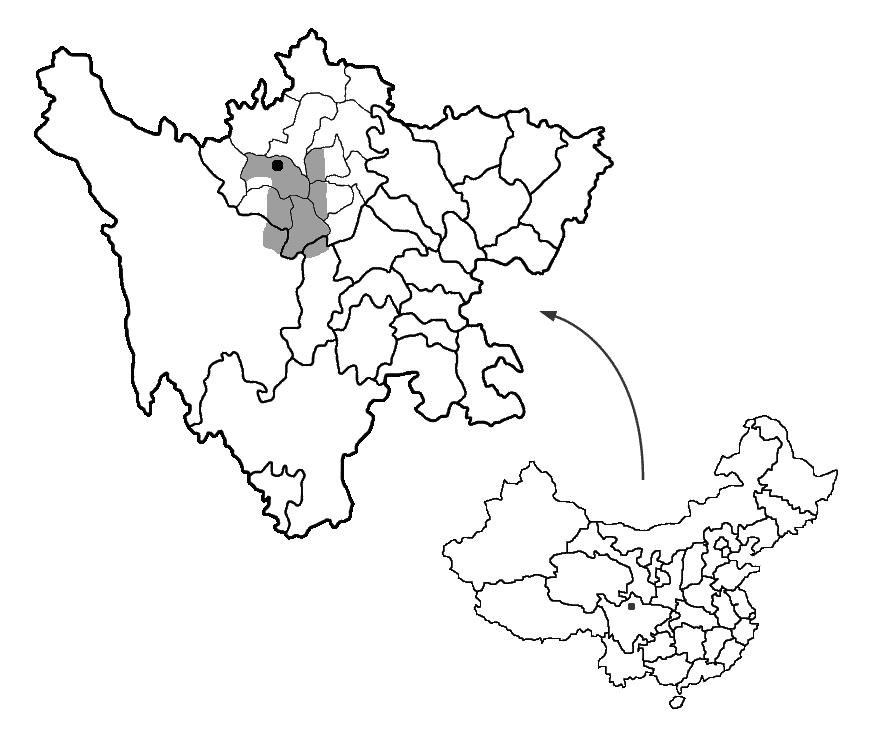
\includegraphics[height=100mm]{carte.JPG}
\caption{Rgyalrong languages}
\label{fig:rgyalrong}
\end{figure}
 

Like other Rgyalrong languages, Japhug presents a very rich system of prefixal voice derivation, including causative, applicative, passive, anticausative, antipassive (\citealt{jacques12demotion}) and incorporation (\citealt{jacques12incorp}); transitive verbs agree with two arguments in person and number.

In this section, we present all background information needed to follow the argumentation: transitivity marking in Japhug, nominal morphology and nominalization. Antipassive derivation in Japhug is described in more detail in section \ref{sec:antipassive}. We will in particular discuss the fact that no less than four different  \ipa{tɯ--} prefixes are found in nouns, a topic that will be of importance for our diachronic hypothesis in section \ref{sec:evidence}.
 
 
\subsection{Nominal morphology} \label{subsec:nominal}
As the present article will discuss the derivation of verbs from nouns, some information on nominal morphology is necessary. Three features of nouns are described here:  possession and number. 


The main morphological feature of Japhug nouns is possession. Nouns can be divided into two main categories: inalienably and alienably possessed nouns.\footnote{This terminology follows works such as \citet{thompson96koyukon}  on Athabaskan languages; see also \citet{jackson98morphology} on the related Tshobdun language.} Inalienably possessed nouns require a possessive prefix in all cases, while alienably possessed nouns may or may not have such a prefix.
            %Unpossessible nouns cannot have an overt possessor without some morphological modifications.

Inalienably possessed nouns must either bear one of the possessive prefixes in Table \ref{tab:pronoun}. The indefinite possessive prefix has two variants \ipa{tɯ}-- and \ipa{tɤ}-- whose distribution  is lexically determined. Alienably possessed nouns can take the prefixes in Table \ref{tab:pronoun}, but not the indefinite possessive prefix. 



\begin{table}[H] \centering
\caption{Pronouns and possessive prefixes }\label{tab:pronoun}
\begin{tabular}{lllllllll} 
\toprule
 Free pronoun & Prefix & Person\\
\midrule
 \ipa{aʑo},    \ipa{ɤj} &	\ipa{a--}  &		1\sg{} \\
\ipa{nɤʑo},  \ipa{nɤj} &	\ipa{nɤ--}  &			2\sg{} \\
\ipa{ɯʑo}  &	\ipa{ɯ--}  &			3\sg{} \\
\ipa{tɕiʑo}  &	\ipa{tɕi--}  &			1\du{} \\
\ipa{ndʑiʑo}  &	\ipa{ndʑi--}  &		2\du{} \\	
\ipa{ʑɤni}  &	\ipa{ndʑi--}  &		3\du{} \\	
\ipa{iʑo}, \ipa{iʑora},   \ipa{iʑɤra}   &	\ipa{i--}  &			1\pl{} \\
\ipa{nɯʑo}, \ipa{nɯʑora},   \ipa{nɯʑɤra}  &	\ipa{nɯ--}  &			2\pl{} \\
\ipa{ʑara}  &	\ipa{nɯ--}  &			3\pl{} \\
\ipa{tɯʑo} & \ipa{tɯ--} or \ipa{tɤ--}/\ipa{ta--} & indefinite / generic\\
\bottomrule
\end{tabular}
\end{table}
In this paper, inalienably possessed nouns will be cited by their root form with a hyphen indicating the obligatory presence of a possessive prefix. Thus \ipa{--jaʁ} `hand' implies that the form *\ipa{jaʁ} on its own is not possible for the meaning `hand', and one will either find the indefinite form \ipa{tɯ-jaʁ} `someone's hand' or a form with a possessive prefix such as \ipa{a-jaʁ} `my hand', \ipa{nɤ-jaʁ} `your hand' etc.


Inalienably possessed nouns (\ref{ex:inal.poss} and \ref{ex:inal.indef}) can be converted to alienably possessed by adding a possessive prefix before the indefinite possessor (example \ref{ex:inal.alienable}).

\begin{exe}
\ex \label{ex:inal.poss}
\gll \ipa{ɯ-ʁrɯ} \\
3\textsc{sg.poss}-horn \\
\glt Its horn
\ex \label{ex:inal.indef}
\gll \ipa{ta-ʁrɯ} \\
\textsc{indef.poss}-horn \\
\glt A horn
\ex \label{ex:inal.alienable}
\gll \ipa{ɯ-ta-ʁrɯ} \\
3\textsc{sg.poss}-\textsc{indef.poss}-horn \\
\glt His horn (the horn taken from an animal)
\end{exe}
            
This phenomenon is not restricted to Rgyalrong languages, but also found in other languages with possessive affixes, such as Athabaskan.\footnote{For instance in Navajo we find a similar opposition between  \ipa{si-tsį'} \textsc{1sg.poss}-flesh `my flesh' and \ipa{she-'a-tsį'} \textsc{1sg.poss}-\textsc{indef.poss}-flesh. `my meat (bought at the marker)' (\citealt[10]{ym87navajo}). The theoretical implications of this phenomenon go beyond this paper.}       
            
Aside from possessive prefixes, an important morphological category occurring in the nominal domain are the numeral prefixes of quantifier nouns (Table \ref{tab:numeral}; only numerals up to 10 are indicated, but all numerals up to one hundred can occur as prefixes). These nouns include measure of time (\ipa{tɯ-xpa} `one year' etc), of length (\ipa{tɯ-tɣa} `one handspan' etc), various quantities (\ipa{tɯ-ɣdɤt} `one section' etc) or classifiers (\ipa{tɯ-rdoʁ} `one piece' etc). 


\begin{table}[H]
\caption{Numerals and numeral prefixes in Japhug} \label{tab:numeral}  \centering
\begin{tabular}{lllllll}
\toprule
&Numeral & prefix \\
\midrule
1 &\ipa{ci} &\ipa{tɯ--} \\
2 &\ipa{ʁnɯz} &\ipa{ʁnɯ--} \\
3 &\ipa{χsɯm} &\ipa{χsɯ--} \\
4 &\ipa{kɯβde} &\ipa{kɯβde-} \\
5 &\ipa{kɯmŋu} &\ipa{kɯmŋu--} \\
6 &\ipa{kɯtʂɤɣ-} &\ipa{kɯtʂɤ--} \\
7 &\ipa{kɯɕnɯz} &\ipa{kɯɕnɯ--} \\
8 &\ipa{kɯrcat} &\ipa{kɯrcɤ-} \\
9 &\ipa{kɯngɯt} &\ipa{kɯngɯ--} \\
10 &\ipa{sqi} &\ipa{sqɯ--} \\
\bottomrule
\end{tabular}
\end{table}

Although the numeral prefix \ipa{tɯ--} is formally similar to the indefinite possessor \ipa{tɯ--}, the two are entirely distinct, as they alternate within different paradigms (respectively Tables \ref{tab:pronoun} and \ref{tab:numeral}). It is not possible to add both series of prefixes on the same quantifier noun. Non-quantifier nouns cannot receive numeral prefixes.  

Numeral prefixes are obligatory with quantifier nouns. The only exception is observed with measures of time: the numeral prefixes can be replaced  with the third person possessive \ipa{ɯ--} to express the meaning `that (particular) year', `that day' etc, as in  example \ref{ex:Wxpa}. 

\begin{exe}
\ex \label{ex:Wxpa}
\gll \ipa{nɯ}   	\ipa{ɯ-xpa}   	\ipa{taχpa}   	\ipa{maka}   	\ipa{mɤ-pe}   	\ipa{tu-ti-nɯ}    \\
\textsc{dem} 3\textsc{sg.poss}-year harvest at.all \textsc{neg-npst}:good \textsc{ipf}-say-\textsc{pl}\\
\glt `People say that the harvest is not good in a year like that.' (Lhamtshams.32)
\end{exe}

No other possessive prefix may be used with these measure nouns.

\subsection{Nominalization} \label{subsec:nmlz}
Japhug Rgyalrong, like other Rgyalrong languages (see for instance \citealt{jackson03caodeng} on the Tshobdun language), has a very rich system of nominalization prefixes. Four different prefixes are productive: the S/A nominalization \ipa{kɯ--}, the O nominalization \ipa{kɤ--}, the oblique nominalization \ipa{sɤ--}  and the action nominalization \ipa{tɯ--}. This section will briefly describe the first three, then describe the prefix \ipa{tɯ}-- and prefixless nominalized forms in more detail, as the latter two will be more relevant to our diachronic hypothesis in section \ref{sec:evidence}.  

\subsubsection{Argument and adjunct nominals} \label{subsubsec:arg}
The nominalized forms derived with the three first prefixes \ipa{kɯ--}, \ipa{kɤ}-- and \ipa{sɤ}-- are  fully productive, and can be used to build relative clauses (\citealt[464-9]{jacques04these}).  The  S/A nominalization prefix \ipa{kɯ--} appears with both intransitive and transitive verbs, but in the latter case a possessive prefix (from Table \ref{tab:pronoun}) coreferent with the patient is added (see \ref{ex:kill}). This nominalized form can be used as one of the tests to determine whether a particular verb is transitive or intransitive (cf section \ref{subsec:trans})

 \begin{exe}
\ex
\gll \ipa{kɯ-si}    \\
  \textsc{nmlz}:S/A-die \\
 \glt  `The dead one'.
 
\ex \label{ex:kill}
\gll \ipa{ɯ-kɯ-sat}    \\
  \textsc{3sg}-\textsc{nmlz}:S/A-kill \\
 \glt  `The one who kills him.'
 \end{exe}


The nominalization prefix \ipa{kɯ}-- has two irregular forms   \ipa{ɣ}-- or \ipa{x}-- which can be found in a few nouns  (Table \ref{tab:irr.nmlz}). Most of these nouns are possessed nouns, but mainly occur with the third person singular possessive \ipa{ɯ}--.

\begin{table}[H]
\caption{Irregular nominalizations in \ipa{ɣ}-- and \ipa{x}--} \label{tab:irr.nmlz} \centering
\begin{tabular}{llll}
\toprule
 noun & meaning &base verb & meaning\\
\midrule
\ipa{\textbf{ɣ}ndʑɤβ} & disastrous fire & \ipa{ndʑɤβ} & burn \\
\ipa{--\textbf{ɣ}ɲaʁ}   &disaster& \ipa{ɲaʁ} & be black \\
\ipa{--\textbf{ɣ}ɲɟɯ}   & orifice & \ipa{ɲɟɯ} & be opened \\
\ipa{--\textbf{x}so}   &  empty thing &\ipa{so} & be empty \\
\bottomrule
\end{tabular}
\end{table}

The semantic relationship between the base verb and the derived nouns in Table \ref{tab:irr.nmlz} is not entirely obvious synchronically, as the nouns have undergone an independent semantic evolution.  The changes from /k/ $\rightarrow$ /ɣ/ and /k/ $\rightarrow$ /x/ on the other hand are perfectly regular in Japhug; the phonological irregularity lies in the loss of the vowel only.

As the first element of a cluster in Japhug, stops only occur before the non-nasal sonorants /r/, /j/, /w/, /l/ and /ɣ/.\footnote{A few minor exceptions are discussed in \citet[45, 261]{jacques04these}, but are of no incidence to the present discussion.}

This gap in the distribution of velar and labial is accounted for if we take into consideration the fact that clusters with velar or labial fricatives as their first element in Japhug always correspond to clusters with velar or labial stops in the closely related Situ language  (\citealt[270]{jacques04these}; for instance,  \ipa{--xtɤɣ} `brother' corresponds to Situ Rgyalrong \ipa{--kték}), which suggests that as the first element of clusters, stops have undergone fricativisation in Japhug. 

Since the language  disallows  clusters of the type stop+nasal as well as stop+s altogether, and since the velar fricatives /x/ and /ɣ/ always agree in voicing with the following consonant in clusters (all other possibilities - *\ipa{kn}--, *\ipa{xn}--, *\ipa{gn}--, are not acceptable clusters in Japhug). Note that irregular nouns in Table \ref{tab:irr.nmlz} are attested for only verbal roots with a simple initial consonant, without any cluster (prenasalized voiced obstruents count as one phoneme in Japhug). This is by no means a coincidence, but rather an effect of the fact that with clusters, the /k--/ prefix would have been dropped without a trace.


Alongside the nouns in table \ref{tab:irr.nmlz}, all four verbs allow the  phonologically and semantically regular corresponding nominalized forms (\ipa{kɯ-ɲaʁ} `the black one', \ipa{kɯ-so} `the empty one' etc), which were regularly created after the irregular nominalizations became opaque. 

The irregular loss of vowels in the examples in table \ref{tab:irr.nmlz} is by no means limited to the nominalization prefix \ipa{kɯ}--, as it is also observed with the animal class prefixes \ipa{kɯ}-- which becomes \ipa{x--}/\ipa{ɣ--}  in some examples but not in others. Comparison with Situ Rgyalrong, which never undergoes vowel loss in prefixes, allows one to detect these examples.

\begin{table}[H]
\caption{Sporadic vowel attrition in the animal class prefixes in Japhug} \label{tab:animal} \centering
\begin{tabular}{llllllllllll}
\toprule
Japhug & meaning & Situ     \\
\midrule
\ipa{kɯ-rtsɤɣ} & leopard & \ipa{kə-ɕtɕík} \\
\ipa{kɯ-ɕpaz} & marmot & \ipa{kʰɐ-ʃpɐ̂s} \\
\midrule
\ipa{ɣ-zɯ} & monkey & \ipa{kə-tsú}\\
\ipa{ɣ-ni} & flying squirrel & \ipa{ka-ɲí}\\
\bottomrule
\end{tabular}
\end{table}
The examples in Table \ref{tab:animal} suggest that vowel attrition only takes place in words whose second syllable has a simple onset (does not begin in an initial cluster), a feature shared with the examples of Table \ref{tab:irr.nmlz}.\footnote{In any case, even if counterexamples to this generalization are found, this would not be surprising, as vowel attrition in presyllables and monosyllabicization tend to be a sporadic process in its first stages (see \citealt{michaud12mono}).}

Vowel attrition of prefixes occurs either with non-productive prefixes such as the animal class prefix or with productive prefixes (such as the S/A nominalization prefix \ipa{kɯ}--) that become reanalysed as a part of the stem due to the semantic evolution of the deverbal noun in question. Another such example is studied in section \ref{subsubsec:action}.



\subsubsection{Action nominals } \label{subsubsec:action}
Beside the argument and adjunct nominalization prefixes studied in the previous subsection, we also find  \textit{action} or \textit{result} nominals in \ipa{tɯ}--. 

The literature on Rgyalrong languages designates these forms as `action nouns' (\citealt[455]{jacques04these}) or `lexicalized action nominals' (\citealt{jacksonlin07}).\footnote{There are two distinct scholarly traditions on this particular topic, \citet{comrie76nmlz} and \citet[5]{koptjevskaja93nmlz} on the one hand who use the terms `action nominal' and `action nominal constructions', and \citealt{grimshaw90argument} on the other hand, whose work focusses on the distinction between \textit{process} and \textit{result} nominals which is not taken into account in \citet{koptjevskaja93nmlz}. We retain here the term `action nominal'; this construction would be labelled as `result nominal' in Grimshaw's framework.}
 
Action nominals can be used to refer to the action or process designated by the verb. They can occur in constructions with a light verb such as  (\ref{ex:light.verb}), or as the complement of the verb \ipa{ʑa} `to begin' (\ref{ex:begin}); both intransitive and transitive verbs can participate in such constructions.

\begin{exe}
\ex \label{ex:light.verb}
\gll \ipa{tɯ-rɟaʁ} \ipa{pɯ-βzu-t-a} \\
\textsc{nmlz:action}-dance \textsc{pfv}-do-\textsc{pst-1sg} \\
%\ex \label{ex:no.light.verb}
%\gll \ipa{pɯ-rɟaʁ-a} \\
%\textsc{pfv}-dance-\textsc{1sg} \\
\glt `I danced.'
\ex \label{ex:begin}
\gll \ipa{ɯ-di}   	\ipa{tɯ-mnɤm}   	\ipa{ta-ʑa}   	\ipa{tɕe}   	\ipa{cʰa}   	\ipa{to-rɤru}   	\ipa{tu-ti-nɯ}   	\ipa{ŋu}   \\
\textsc{3sg.poss}-smell \textsc{nmlz:action}-smell \textsc{pfv:3$\rightarrow$3}-begin \textsc{lnk} alcohol \textsc{evd}-get.up \textsc{ipfv}-say-\textsc{pl} \textsc{npst}:be \\
\glt `When it starts to smell, people say `the alcohol has fermented'.' (Alcohol, 77)
\end{exe} 

Action nominals cannot take any TAM markers but  can receive possessive prefixes. However, the possessor does not   necessarily correspond to any of the arguments of the original verb. For instance, in the case of the noun \ipa{tɯ-rɟaʁ} `a dance' derived from the intransitive \ipa{rɟaʁ} `to dance', possessive prefixes as in  \ipa{ɯ-tɯ-rɟaʁ} `his dance' are generally interpreted as the beneficiary of the action, not the dancer (`a dance performed in his honour').



With stative verbs, \ipa{tɯ}-- nominals express the abstract property of the verb (like the derivation of  nouns from adjectives by the suffix --\textit{ness} in English) and are better labelled as `property nominals'.  \ipa{tɯ}-- nominals  commonly occur in a degree construction, followed by another stative verb indicating degree such as \ipa{saχaʁ} `to be extremely ...' or \ipa{sɤre} `to be ridiculous, to be terribly ...'.
\begin{exe}
\ex
\gll \ipa{βɣɯz}   	\ipa{nɯ}   	\ipa{li}   	\ipa{ɯ-di}   	\ipa{ɯ-tɯ-sɤjloʁ}   	\ipa{sɤre}   	\ipa{ʑo}   \\
badger \textsc{top} too \textsc{3sg.poss}-smell \textsc{3sg.poss}-\textsc{nmlz:property}-awful \textsc{npst}:terrible \textsc{emph} \\
\glt `The badger's smell is awful.' (`the badger's smell's awfulness is terrible')
\end{exe}

 
Unlike the argument nominals discussed in the previous subsection,   \ipa{tɯ}-- action nominal derivation is not fully productive, and the semantics of the action nominals is not always predictable. In some cases, it refers  to the \textit{result of the action} rather than the action itself (thus \ipa{tɯ-taʁ} `woven cloth' from \ipa{taʁ} `to weave') or even the object of the action (\ipa{tɯ-tsʰi} `rice porridge' from \ipa{tsʰi} `to drink') and the semantics of the noun is not always predictable and tends to be more specific than that of the verb. It is however cross-linguistically quite common for action nominals to  present this kind of irregular semantics for some nouns (\citealt[20-21]{koptjevskaja93nmlz}). 

Table \ref{tab:irr.act.nmlz} illustrates the most representative examples of such irregular nouns. Apart from numerous examples with irregular semantics, we also find two examples with irregular phonology. 

\begin{table}[H]
\caption{Examples of irregular action nominals and their base verbs} \label{tab:irr.act.nmlz}
\begin{tabular}{llllll}
\toprule
 noun & meaning &base verb & meaning& irregularity\\
\midrule
\ipa{tɯsqa}   &wheat porridge& \ipa{sqa} & cook & semantics \\
\ipa{tɯpu}   &moxibustion& \ipa{pu} & cook in ashes &id.\\
\ipa{tɯpɣaʁ}   &land reclamation& \ipa{pɣaʁ} & turn over &id.\\
\midrule
\ipa{tɯtsɣe}&commerce & \ipa{ntsɣe} & sell & phonology\\
\ipa{--nŋa}   &debt& \ipa{ŋa} & owe &id.\\
\bottomrule
\end{tabular}
\end{table}

In the following, we provide a detailed account of one action nominal with irregular semantics (\ipa{tɯpɣaʁ}   `land reclamation') as well as of the the two action nominals with irregular phonology. These three examples will be relevant to our hypothesis on the origin of the antipassive in section \ref{sec:evidence}.

\paragraph{Irregular semantics}

The transitive  \ipa{pɣaʁ} `to turn around, turn over' has numerous meanings. It can be applied to sheet-like objects, and with clothes it can even mean `to wear inside out'. It has other specialized meanings like `to cross a mountain', `open the cover/lid' or `to plough a field', with different directional prefixes.
 
   \begin{exe} \label{ex:topGaR}
\ex
\gll  \ipa{ndʑi-pʰɤrtʰɤβ}    	\ipa{nɯ}    	\ipa{tɕu,}    	\ipa{jɤlwa}    	\ipa{ci}    	\ipa{pjɤ-tu}    	\ipa{tɕɤn,}    	\ipa{nɯ}    	\ipa{qale}    	\ipa{ci}    	\ipa{kɯ}    	\ipa{to-pɣaʁ}    \ipa{ri} \\
\textsc{3du.poss}-between \textsc{top} \textsc{loc} curtain one \textsc{evd.ipfv}-exist \textsc{coord} \textsc{dem} wind one \textsc{erg} \textsc{evd}-turn.over but \\
 \glt `Between them, there was a curtain, and a wind turned it over.' (The frog, 98)
\end{exe} 

   \begin{exe} \label{ex:tapGaR}
\ex
\gll   \ipa{ɯ-fkaβ} \ipa{ta-pɣaʁ} \\
 \textsc{3sg.poss}-cover \textsc{pfv:3$\rightarrow$3:up}-turn.over \\
 \glt  `He opened the cover.' (Lobzang, 49)
\end{exe} 


The meaning `to plough' is always associated with directional prefixes indicating the `upstream' direction (the same as all verbs meaning `to dig' in the language):
   \begin{exe} \label{ex:lapGaR}
\ex
\gll   \ipa{tɯji} \ipa{la-pɣaʁ} \\
field \textsc{pfv:3$\rightarrow$3:upstream}-turn.over \\
 \glt  `He ploughed the field.'
\end{exe} 

On the other hand, the nominalized form of the verb only has one meaning: the action of reclaiming land by ploughing for the first time (in Chinese \zh{开荒} \textit{kaihuang}), as illustrated by the following example from the Flood myth:

\begin{exe} \label{ex:tWpGaR}
\ex
\gll   \ipa{tɯ-pɣaʁ} \ipa{lo-tɕɤt-ndʑi} \\
\textsc{nmlz:action}-turn.over \textsc{evd:upstream}-take.out-\textsc{du} \\
 \glt  `They^{du} reclaimed land.' (The flood, 85)
\end{exe}

\paragraph{Irregular phonology}
As the argument nominals discussed in \ref{subsubsec:arg}, there are also a few action nominals with irregular phonology. 

First, the transitive verb \ipa{ntsɣe} `to sell' has an  action noun \ipa{tɯtsɣe} `commerce'  which presents a stem /\ipa{tsɣe}/ distinct from that of the base verb in lacking a \ipa{n--}. An explanation for the additional \ipa{n}-- in  \ipa{ntsɣe} `to sell' will be proposed in section \ref{sec:appl}.

Second,  the possessed noun \ipa{--nŋa} `debt' appears to be related to the verb \ipa{ŋa} `to owe' but it lacks a derivational \ipa{tɯ}-- prefix and has a additional \ipa{n}-- element.\footnote{Since \ipa{--nŋa} is a inalienably possessed noun, its form without definite possessive prefix is \ipa{tɯ-nŋa}, but the \ipa{tɯ--} here is the indefinite possessor prefix, and alternates with the series of possessive prefix in Table \ref{tab:pronoun}. } In the following, we will show that this \ipa{n--} is a trace of the derivational \ipa{tɯ}-- prefix.

We saw in section \ref{subsubsec:arg} (Table \ref{tab:irr.nmlz}) that irregular argument nominals were formed by deleting the vowel of the derivational prefix and applying automatic phonological changes to the prefixed stop (\ipa{kɯ}-- becomes \ipa{ɣ}-- or \ipa{x}-- in these nouns). We mentioned that comparative evidence with Situ Rgyalrong indicate that velar and labial stops underwent fricativization in Japhug when occurring as first member of  clusters having an obstruent as   second member. In the case of coronal stops however, clusters with /t/ or /d/ followed by a consonant other than a non-nasal sonorant exist in Japhug in internal position (though mainly in loanwords from Tibetan across morpheme boundaries).

Let us now observe the synchronic distribution of clusters which have a nasal as second member in Japhug (data from \citealt{jacques04these}).

\begin{table}[H]
\caption{Clusters with a nasal as a second member in Japhug}  \label{tab:nasal} \centering
\begin{tabular}{llllll}
\toprule
  &  	labial  &  	dental  &  	velar  \\  
  \midrule
labial  &  	\grise{}  &  	\ipa{mn--}  &  	\ipa{mŋ--}  \\  
dental  &  	\ipa{nm--}  &  	\grise{}  &  	\ipa{nŋ--}  \\  
velar  &  	\ipa{ɣm--}  &  	\ipa{ɣn--}  &  	\grise{}  \\  
\bottomrule
\end{tabular}
\end{table}

We see that there are no clusters with a nasal velar as the first element (*\ipa{ŋm}--, *\ipa{ŋn}--) but that on the other hand there are no clusters with a dental or a labial non-nasal (*\ipa{βn}--, *\ipa{tn}--). Moreover, \ipa{n}-- as the first element of a cluster has a very restricted distribution. It occurs only (i) before a coronal stop or affricate (clusters such as /\ipa{ntʰ--}/, /\ipa{nts--}/ etc, where it is the realization of the homorganic nasal archiphoneme /N/), (ii) before voiced prenasalized stops (/\ipa{nmb}/ and /\ipa{nŋg}/, transcribed as \ipa{nb--} and \ipa{ng--} in this work) (iii) before nasal consonants (the examples in Table \ref{tab:nasal}). \ipa{n}-- is conspicuously absent as the first element of a cluster before labial  and velar stops (outside of the voiced prenasalized one). Thus, one does not find clusters such as *\ipa{np--} or *\ipa{nkʰ--} in Japhug. 

If \ipa{n}-- as first element of a cluster in cases (ii) and (iii) originated from *n-- in pre-Japhug, there would be no reason why only \ipa{nmb--} and \ipa{nm--} are possible while *\ipa{np--} and *\ipa{npʰ--} are not. A solution to this paradox is to assume that \ipa{n--} in cases (ii) and (iii) originate from */t/, which underwent retrograde nasality assimilation, as indicated in table \ref{tab:assimilation}.

\begin{table}[H]
\caption{Retrograde nasality assimilation in Japhug clusters} \label{tab:assimilation} \centering
\begin{tabular}{lllll}
\toprule
pre-Japhug & Japhug \\
\midrule
\ipa{*tm}-- & \ipa{nm--} \\
\ipa{*tŋ}-- & \ipa{nŋ--} \\
\ipa{*tmb}-- & \ipa{nb--} \\
\ipa{*tŋg}-- & \ipa{ng--} \\
\bottomrule
\end{tabular}
\end{table}
The best evidence for  this sound law comes from loanwords from Tibetan, where internal t+nasal clusters automatically undergo these changes (for instance Tibetan \ipa{mtɕʰod.me} `traditional lamp' and \ipa{rgod.ma} `mare' were borrowed as \ipa{mtɕʰɤnmi} and \ipa{rgonma}).\footnote{The Tibetan translitteration used here follows \citet{jacques12transcription}. }

Thus, equipped with this sound law,  it is possible to reconstruct \ipa{--nŋa} `debt' as *\ipa{tŋa} in pre-Japhug, a form coming from the expected regular form *\ipa{tɯŋa} by loss of the vowel. This is the only known case in Japhug when a action nominal prefix \ipa{tɯ}-- undergoes irregular vowel loss.



%tsʰɤrme

This particular example will be relevant to our discussion in section \ref{sec:evidence} on the origin of the antipassive in Japhug.

\subsubsection{Bare infinitive  and derived inalienably possessed nouns} \label{subsubsec:bare}
Besides \ipa{tɯ}-- prefixed nominals, we also find another type of action nominal:   bare  infinitives. These non-finite forms are formed by combining the bare base stem with a possessive prefix coreferent with the patient, as \ipa{ɯ-mto} in (\ref{ex:bare.inf}). Only transitive verbs can form bare infinitives (intransitive verbs use \ipa{kɤ}-- prefixed forms in the same contexts).

\begin{exe}
\ex \label{ex:bare.inf}
\gll \ipa{nɤʑo} 	\ipa{kɯ-fse} 	\ipa{a-ŋkʰor} 	\ipa{nɯ} 	\ipa{ɯ-mto} 	\ipa{mɯ-pɯ-rɲo-t-a} \\
you \textsc{nmlz:stative}-be.like \textsc{1sg.poss}-subject \textsc{top} \textsc{3sg}-\textsc{bare.inf:}see \textsc{neg-pfv}-experience-\textsc{pst:tr-1sg} \\
\glt  `I never saw anyone like you among my subjects.' (Smanmi metog koshana1.157)
\end{exe}

We also find bare infinitives instead of action nominals with the verb \ipa{ʑa} `to start' when the patient is an overt noun phrase, as in example \ref{ex:bare.inf.za}.

\begin{exe}
\ex \label{ex:bare.inf.za}
\gll \ipa{tɤscoz} 	\ipa{ɯ-rɤt} 	\ipa{pa-ʑa} 	  \\
letter \textsc{3sg.poss}-\textsc{bare.inf:}write \textsc{pfv:3$\rightarrow$3}-start\\
\glt  `He started writing a letter.' (elicited)
\end{exe}

 
The bare infinitive can also be used as an action nominal in combination with the noun \ipa{tsʰɯɣa} `form, appearance' as in example (\ref{ex:bare.inf.noun}).

\begin{exe}
\ex \label{ex:bare.inf.noun}
\gll \ipa{ndʑi-mi}   	\ipa{ɯ-tsʰoʁ}   	\ipa{ɯ-tsʰɯɣa}   	\ipa{nɯra}   	\ipa{wuma}   	\ipa{ʑo}   	\ipa{naχtɕɯɣ-ndʑi.}   \\
\textsc{3du.poss}-foot \textsc{3sg}-\textsc{bare.inf:}attach.to \textsc{3sg.poss}-form \textsc{top:pl} very \textsc{emph}  \textsc{npst}:similar-\textsc{du}  \\
\glt `The way their feet (of fleas and crickets) touch the ground is very similar.' (the cricket 17)
\end{exe}

In addition to bare infinitives, there is a rarer formation of bare action nominalizations by prefixation of possessive prefixes to the bare stem of verbs; the indefinite possessor is either \ipa{tɯ}-- or \ipa{tɤ}-- (Table \ref{tab:nmlz-inalienably}). 

\begin{table}[H]
\caption{Bare nominalizations (inalienably possessed nouns)} \label{tab:nmlz-inalienably}
\begin{tabular}{llllllllll}
\toprule
base verb & meaning & noun stem & indefinite  & meaning\\
&&&possessor\\
\midrule
\ipa{fkaβ} & cover& \ipa{--fkaβ} & \ipa{tɤ-fkaβ} & lid\\
\ipa{ɕpʰɤt} & patch& \ipa{--ɕpʰɤt} & \ipa{tɤ-ɕpʰɤt} & patch (n.) \\
\ipa{sɯso} & think & \ipa{--sɯso} & \ipa{tɯ-sɯso} & thought \\
\bottomrule
\end{tabular}
\end{table}

Given the absence of morphemes other than the possessive prefixes, it is legitimate to wonder whether the direction of derivation in the examples in Table \ref{tab:nmlz-inalienably} is indeed from verb to noun as posited here. The proof that this is indeed the correct direction of derivation is the fact that the verb \ipa{fkaβ} `to cover' is borrowed from Tibetan \ipa{bkab}, the past tense form of the verb \ipa{ⁿgebs} `to cover'. The noun \ipa{--fkaβ} `cover' is clearly secondary and was created within Japhug, as there is no such corresponding noun in Tibetan.

  
\subsection{Transitivity in Japhug} \label{subsec:trans}
Since the focus of this paper is on valency-decreasing derivation, it is necessary to provide some information on transitivity marking in Japhug. 
Japhug, like all Rgyalrong languages, has a very clear   distinction between transitive and intransitive verbs, which is reflected in both case marking and verbal morphology. Morphological transitivity is unambiguous and  marked in   different but congruent  ways, some of which have been mentioned above.

First,  Japhug  is a strongly head-marking language, with person and number of both arguments marked on the verb (\citealt{jacques10inverse}). Only transitive verbs can receive the inverse prefix \ipa{wɣɯ}--, the portmanteau prefixes \ipa{kɯ}-- (2$\rightarrow$1), \ipa{ta}-- (1$\rightarrow$2), the perfective direct 3$\rightarrow$3'  \ipa{a}-- prefix or  the 1/\textsc{2sg}$\rightarrow$3 --\ipa{t} suffix (the latter only occurs in open-syllable stem verbs).


Second, Japhug has ergative flagging:  S and P are unmarked (examples \ref{ex:abs} and \ref{ex:erg}) , while the A of a transitive verb receives the clitic \ipa{kɯ} (example \ref{ex:erg}). This clitic is obligatory with nouns and third person pronouns, but optional for first and second person pronouns. The \ipa{kɯ} clitic can also be used to mark instruments.

\begin{exe}
\ex \label{ex:abs}
\gll \ipa{tɤ-tɕɯ}  	\ipa{nɯ}  	 	\ipa{jo-ɕe}   \\
\textsc{indef.poss}-boy \textsc{top}   \textsc{evd}-go \\
\glt `The boy went (there).'
\end{exe}

\begin{exe}
\ex \label{ex:erg}
\gll \ipa{tɤ-tɕɯ}  	\ipa{nɯ}  	\ipa{kɯ}  	\ipa{χsɤr}  	\ipa{qaɕpa}  	\ipa{nɯ}  	\ipa{cʰɤ-mqlaʁ}   \\
\textsc{indef.poss}-boy \textsc{top} \textsc{erg} gold frog \textsc{top} \textsc{evd}-swallow \\
\glt  The boy swallowed the golden frog.' (Nyima Wodzer.1, 131)
\end{exe}

Third,  some transitive verbs present a special stem in direct \textsc{123sg}$\rightarrow$3 forms. The regular pattern is that verbs whose stem is in --\ipa{o}, --\ipa{u}, --\ipa{a} and --\ipa{ɯ} change to --\ipa{ɤm}, --\ipa{e}, --\ipa{e} and --\ipa{i} respectively. This stem alternation does not occur with intransitive verbs.

Fourth, argument nominalisation of transitive   and intransitive  verbs present tripartite alignment, as the S nominalization is marked by \ipa{kɯ}--, while A nominalization is marked by a possessive prefix followed \ipa{kɯ}-- and P-nominalization by \ipa{kɤ}-- (section \ref{subsubsec:action}). Argument nominalization can therefore always be used to distinguish transitive from intransitive verbs.


There are a few labile verbs is Japhug, and all present agent-preserving ambitransitivity  (\citealt[217-9]{jacques12demotion}). When used intransitively, labile verbs are interpreted as having an undefined patient, as in example (\ref{ex:pWtaR}).

 \begin{exe}
\ex \label{ex:pWtaR}
\gll  \ipa{tɕʰeme} 	\ipa{ci} 	\ipa{pɯ-taʁ} 	\ipa{ɲɯ-ŋu}  \\
girl \textsc{indef} \textsc{pst.ipf}-weave \textsc{const}-be \\
\glt `A girl was weaving.' (The demon, 28)
 \end{exe}
 
Non-overt patients of non-labile transitive verbs on the other are always interpreted  as a referent previously mentioned in the text. Thus,  in a sentence such as \ref{ex:def}, the verb \ipa{tu-ndze} (\textsc{ipf}-eat[III]) can only mean `eat it', never `eat something'.\footnote{In this particular example, the non-overt patient is \textit{mice} as a species, which were referred to previously in the text; in Japhug generic referents can be either singular or plural.}

\begin{exe}
\ex \label{ex:def}
\gll  \ipa{tɯji} 	\ipa{ɯ-ngɯ} 	\ipa{tɕe,} 	\ipa{qapri} 	\ipa{kɯ} 	\ipa{tu-ndze} 	\ipa{ŋgrɤl} 	\ipa{tɕe,} 						
\ipa{kha} 	\ipa{tɕe} 	\ipa{lɯlu} 	\ipa{kɯ} 	\ipa{tu-ndze} 	\ipa{ŋu} 	    \\
field \textsc{3sg.poss}-inside \textsc{lnk} snake \textsc{erg} \textsc{ipf}-eat[III] \textsc{npst}:be.usually.the.case \textsc{lnk} house  \textsc{lnk}  cat \textsc{erg} \textsc{ipf}-eat[III] \textsc{npst}:be \\
\glt `In the field,   snakes  eat  them (mice) and in the house,    cats eat  them.'  (Mice, 163-4) 
\end{exe}

 
There are three ways to have an unspecified patient with a non-labile transitive verb.  First,  the generic human marker \ipa{kɯ}-- can be prefixed to the verb.\footnote{The generic marker for S and P in Japhug is \ipa{kɯ}--, a prefix unrelated at least synchronically to the homophonous nominalization prefix \ipa{kɯ}--  (\citealt[204-89]{jacques12demotion}). Generic marking in Japhug will not be discussed in this paper. Unlike human antipassive, generic patients in \ipa{kɯ}-- can be topical, and this form is typically used in gnomic statements and procedural texts.} Second,  an indefinite pronoun such as \ipa{tʰɯci} `something' can be used. Third, the verb can be intransitivized by means of an antipassive prefix.



Example \ref{ex:akAkWmtsWG} illustrates a switch of use between the   antipassive \ipa{sɤ}-- and the generic \ipa{kɯ}-- across two sentences.

\begin{exe}
\ex \label{ex:akAkWmtsWG}
\gll
\ipa{nɯ} 	\ipa{aʁɤndɯndɤt} 	\ipa{ɯ-grɤl} 	\ipa{kɯ-me} 	\ipa{kɯ-sɤ-mtsɯɣ} 	\ipa{ɲɯ-ŋu.} 
 \ipa{nɯ} 	\ipa{kɯ} 	\ipa{a-kɤ-kɯ-mtsɯɣ} 	\ipa{tɕe} 	\ipa{tɕe} 	\ipa{nɯ} 	\ipa{ɯ-tɯɣ} 	\ipa{ɣɤʑu.} \ipa{tɕe} 	\ipa{tɯʑo} 	\ipa{ɲɯ-kɯ-ɕte} 	\ipa{ɲɯ-ŋu.} 
 \\
 \textsc{dem} everywhere \textsc{3sg.poss}-order \textsc{nmlz}:S/A-not.exist \textsc{nmlz}:S/A-\textsc{antipass:human}-bite \textsc{const}-be \textsc{dem} \textsc{erg} \textsc{irr-pfv-genr}:S/P-bite \textsc{lnk} \textsc{lnk} \textsc{dem} \textsc{3sg.poss}-poison \textsc{sensory}:exist \textsc{lnk} \textsc{generic} \textsc{ipfv-genr}:S/P-infect \textsc{const}-be\\ 
\glt `(Rabid dogs)  bite people without discrimination, and if one is bitten by them, there is poison (in their bites) and one gets infected.'  (Rabies, 8)
\end{exe}

This sentence shows that using   the generic form allows anaphoric reference (the P of the verbs \ipa{a-kɤ-kɯ-mtsɯɣ} `if one is bitten' and  	\ipa{ɲɯ-kɯ-ɕte}   `one gets infected' must be the same generic referent), while the antipassive implies that the deleted P is not identifiable  (on this topic see \citealt[52]{cooreman94antipassive}) and no anaphoric reference is possible.

\section{Antipassive in Japhug} \label{sec:antipassive}
Two productive antipassive prefixes are found in Japhug: \ipa{rɤ}-- and \ipa{sɤ}--.\footnote{There is a third antipassive prefix \ipa{ɕɯm}-- only attested with the verb \ipa{tʰu} `to ask' $\rightarrow$ \ipa{ɕɯmtʰu} `to ask a lot of questions'. }  The former is used to delete a non--human patient (\ipa{ɕar} `to search' $\rightarrow$ \ipa{rɤ-ɕar} `to search for things') while the second is used to delete a human patient (\ipa{ɕar} `to search' $\rightarrow$ \ipa{sɤ-ɕar} `to search for people').\footnote{A similar situation is found in the closely related language Tshobdun, (\citealt[8]{jackson06paisheng}), and a typological parallel is observed in Nahuatl which also has a human antipassive \ipa{tē}-- and a non-human antipassive \ipa{tla}-- (\citealt[91]{creissels06sgit2}).}  The patient cannot be reintroduced with oblique case in Japhug antipassive constructions, except for some ditransitive verbs (\ref{subsec:ditr}) . Labile verbs cannot form antipassives.

As illustrated in table \ref{tab:antipassive.jpg}, the formation of the non-human \ipa{rɤ}-- antipassive is perfectly regular (it has an allomorph \ipa{ra}-- before a uvular fricative in closed syllables), except for the verbs \ipa{ŋa} `to owe'' and \ipa{ntsɣe} `to sell',   the first of which is discussed in detail  in section \ref{subsec:phono.irr}. % and \ref{sec:appl}.

\begin{table}[H]
\caption{Examples of the antipassive prefix  \ipa{rɤ}--} \label{tab:antipassive.jpg}
\begin{tabular}{lllllllll} \toprule
\multicolumn{2}{c}{basic  transitive verb}  & \multicolumn{2}{c}{derived  intransitive verb}  \\
\midrule
\ipa{roʁ}   &	to carve &  	\ipa{rɤ-roʁ}   &	to carve things \\  
\ipa{tɕɤβ}   &	to burn &  	\ipa{rɤ-tɕɤβ}   &	to burn land \\  
\ipa{ɕpʰɤt}   &	to patch &  	\ipa{rɤ-ɕpʰɤt}   &	to patch things \\  
\ipa{pɣaʁ}   &	to turn over &  	\ipa{rɤ-pɣaʁ}   &	to reclaim land \\  
\ipa{tʂɯβ}   &	to sew &  	\ipa{rɤ-tʂɯβ}   &	 to sew things \\   
\ipa{ɕar}   &	to search &  	\ipa{rɤ-ɕar}   &	to search for things \\ 
\ipa{ŋa}   &	to owe  (a specific quantity)&  	\ipa{rɤ-nŋa}   &	to owe money \\  
\ipa{ntsɣe}   &	to sell &  	\ipa{rɤ-tsɣe}   &	to sell things \\  
\ipa{χtɯ}   &	to buy &  	\ipa{ra-χtɯ}   &	to buy things \\  
\bottomrule
\end{tabular}
\end{table}


The non-human antipassive \ipa{rɤ}-- detransitivizes transitive verbs, and the S of the derived verb corresponds to the A of the base verb: this is an agent-preserving derivation, unlike the passive and anticausative. The verb takes an intransitive conjugation and the S   appears without ergative marking:

  \begin{exe}
\ex
\gll \ipa{tɤ-rʑaβ} 	\ipa{nɯ} 	\ipa{pjɤ-rɤ-ɕpʰɤt}   \\
    \textsc{indef.poss}-wife \textsc{top} \textsc{evd-antipass:non.human}-mend \\
 \glt    `The wife mended (clothes).' (The raven 19)
\end{exe} 


The human antipassive \ipa{sɤ}-- prefix   presents the allomorph \ipa{sa}-- before a uvular fricative in closed syllables  and the optional variant \ipa{sɤz}-- in a few verbs whose stem begins in \ipa{ɣɤ--}.


\begin{table}[H]
\caption{Examples of the antipassive prefix \ipa{sɤ}--}\label{tab:antipassive.jpg2}
% \resizebox{\columnwidth}{!}{
\begin{tabular}{lllllllll} \toprule
\multicolumn{2}{c}{basic transitive verb} &\multicolumn{2}{c}{derived  intransitive verb}\\
\midrule
\ipa{ɣɤmɯ}   &	to praise &  	\ipa{sɤ-ɣɤmɯ, sɤz-ɣɤmɯ}   & to praise people\\  
\ipa{ɕar}   &	to search &  	\ipa{sɤ-ɕar}   &to search for people \\ 
\ipa{tɕʰɯ}   &	to gore &  	\ipa{sɤ-tɕʰɯ}  & to gore people \\  
\ipa{mtsɯɣ}   &	to bite &  	\ipa{sɤ-mtsɯɣ}  & to bite people  \\  
\ipa{nɤmtsioʁ}   &	to peck &  	\ipa{sɤ-nɤmtsioʁ}    & to peck at people\\  
\ipa{ʁndɯ}   &	to hit &  	\ipa{sa-ʁndɯ}   &	to hit people    \\  
\bottomrule
\end{tabular}
\end{table}

 
In the closely related Tshobdun language, \citet{jackson13morpho} reports two distinct patient-suppressing \ipa{sɐ}-- prefixes,\footnote{\ipa{sɐ}-- in Tshobdun is the form regularly corresponding to Japhug \ipa{sɤ}--.} the human antipassive \ipa{sɐ}-- (deriving action verbs, as \ipa{ntʃʰe} `to kill' $\rightarrow$ \ipa{sɐ́-ntʃʰe} `to do killing (of people)') and a prefix \ipa{sɐ}-- deriving stative verbs meaning `to have a propensity for V-ing' (\ipa{tʃʰuʔ} `to gore' $\rightarrow$ \ipa{sɐ-tʃʰuʔ} `to have a propensity for goring (people)').

In Japhug, the situation is very similar to that of Tshobdun, but it is unclear whether two distinct prefixes must be posited. Human antipassive verbs can be either action verbs or propensity stative verbs depending on the context.

For instance, the human antipassive \ipa{sɤ-sat} of the transitive verb \ipa{sat} `to kill' can be both used as a propensity stative verb  \ipa{sɤ-sat} `have a killing power' (example \ref{ex:sasat1}) or as an action verb `to kill people' (examples \ref{ex:sasat2} and \ref{ex:sasat3}). It should be noted that the implied patient of   propensity stative verbs is generally human, but in some cases can be applied to animals as well. For instance   \ipa{sɤ-sat}  `have a killing power' can designate the killing of both animals or   people.

    \begin{exe} 
\ex \label{ex:sasat1}
\gll  \ipa{nɯnɯ} \ipa{wuma} \ipa{ʑo} \ipa{ɲɯ-sɤ-sat}  \\
  this very \textsc{emph} \textsc{const-antipass:human}-kill \\
 \glt   `Its killing power is considerable (of a gun).' (Guns, 117)
\end{exe}    
 
     \begin{exe} 
\ex \label{ex:sasat2}
\gll  \ipa{kɤ-sɤ-sat}  \ipa{pjɤ-rɲo}\\
   \textsc{inf-antipass:human}-kill \textsc{evd}-experience \\
 \glt  `He has killed [a man] before.' (In Chinese: \zh{他杀过人})
 \end{exe}
      \begin{exe} 
 \ex \label{ex:sasat3}
\gll  \ipa{kɯ-sɤ-sat}  \ipa{jo-ɕe}\\
   \textsc{nmlz:S/A-antipass:human}-kill \textsc{evd}-go \\
 \glt  `He went to kill [people].'
\end{exe} 

In general, human antipassive verbs appear to allow both meanings. For instance, the antipassive \ipa{sɤ-mtsɯɣ} derived from \ipa{mtsɯɣ} `to bite' means both `to have a propensity for biting people' and `to bite people' depending on the context. Depending on the meaning of the base verb, some human antipassive verbs will more commonly tend to be  action verbs; for instance, \ipa{sɤ-ɕar}, the antipassive of \ipa{ɕar} `to search', is usually an action verb `to search for people' and cannot really be interpreted as meaning `to have a propensity for searching for people' but this is probably more for pragmatic reasons than morphosyntactic ones.  

Thus, we will not distinguish in this paper the action human antipassive from the stative antipassive, as this distinction in Japhug reflects specific uses of a single derivation rather than distinct derivations. The tendency of the antipassive construction to express repeated or habitual action rather than a punctual event
is well attested cross-linguistically (cf \citealt[91-2]{cooreman94antipassive}).


\subsection{Compatibility with other derivational prefixes} \label{subsec:compatibility}

\citealt{jacques12incorp} describes the Japhug verb  in terms of    the template in Table \ref{tab:template:derivational} (\citealt{jacques12incorp}). This table represents finite verb forms. In nominalizations, the prefixal slots 1, 5, 6 and all suffixal slots, which mark TAM and person, cannot be filled. Nominalization prefixes described in \ref{subsec:nmlz} always occur between slots 4 and 5.


   \begin{landscape}
\begin{table}[h]
\caption{The Japhug verbal template (shaded areas indicate derivational prefixes)}\label{tab:template:derivational}
\begin{tabular}{llllll|llllllll|lllll} \toprule
 
\ipab{a-}  &  	\ipab{mɯ- }   &  	\ipab{ɕɯ-}   &\ipab{tɤ-} &  	\ipab{tɯ-}  &  	\ipab{wɣ-}   &

  	 \grise{\ipab{ʑɣɤ-}}  &  	\grise{\ipab{sɯ-}}  & \grise{\ipab{rɤ-}}& \grise{\ipab{nɤ-}} &   	 \grise{\ipab{a-}}   &  	\grise{\ipab{nɯ-}}  &  	\grise{\ipab{ɣɤ-}}  &  	\grise{\ipab{noun}}    &  	 \begin{math}\Sigma\end{math}    &  	\ipab{-t}  &  	\ipab{-a}  &  	\ipab{-nɯ}   &  \\
   &  	\ipab{mɤ-}   &  	\ipab{ɣɯ-}   &\ipab{pɯ-}&  	  &  	 
    & \grise{ }	  &  	 \grise{ }	  &  	  \grise{ }	  &  	   \grise{ }	&  	\grise{\ipab{sɤ-}}&  \grise{ }	 &  	\grise{\ipab{rɯ-}}  &  	 \grise{ }	  &  	  &  	  &  	  &  	\ipab{-ndʑi} &  \\
  &  	   &     &  etc.	  & & 	  &  	  &  	 & &  	  &  	 & &  etc.	  &  	  &  	  &  	  &  	  &  	  &  \\
1  &  	2  &  	3  &  	4  &  	5  &  	6  &  	7  &  	8  &  	9  &  	10  &  	11  &  	12  &  	13  &  	14  &  	15  & 16 &17&18\\
\bottomrule
\end{tabular}
\end{table}
\begin{multicols}{2}
\begin{enumerate}


\item Irrealis  \ipa{a}-- and \ipa{ɯβrɤ}--, Interrogative \ipa{ɯ́}--, conative \ipa{jɯ}--
\item negation \ipa{ma}-- / \ipa{mɤ}-- / \ipa{mɯ}-- / \ipa{mɯ́j}--
\item Associated motion \ipa{ɕɯ}-- and \ipa{ɣɯ}--
\item Directional prefixes ( \ipa{tɤ}--  \ipa{pɯ}--  \ipa{lɤ}--   \ipa{tʰɯ}--  \ipa{kɤ}--   \ipa{nɯ}--   \ipa{jɤ}-- ,  \ipa{tu}--   \ipa{pjɯ}--   \ipa{lu}--   \ipa{cʰɯ}--   \ipa{ku}--   \ipa{ɲɯ}--   \ipa{ju}-- ) permansive  \ipa{nɯ}-, apprehensive \ipa{ɕɯ}-
\item Second person (\ipa{tɯ}--, \ipa{kɯ}-- 2$\rightarrow$1 and ta- 1$\rightarrow$2)
\item Inverse -\ipa{wɣ}- / Generic S/O prefix \ipa{kɯ}-, Autobenefactive \ipa{nɯ--}, Progressive \ipa{asɯ}-. The inverse and the autobenefactive can be infixed within the progressive \ipa{asɯ}-.
\item Reflexive \ipa{ʑɣɤ}-- 
\item Causative \ipa{sɯ}--, Abilitative \ipa{sɯ}--
\item \textbf{ Antipassive  \ipa{sɤ}-- / \ipa{rɤ}--}
\item  Tropative \ipa{nɤ}--, applicative \ipa{nɯ}--
\item Passive or Intransitive thematic marker \ipa{a}-- / De-experiencer \ipa{sɤ}--
\item Autobenefactive-spontaneous (appears in this position only when the passive/intransitive determiner is present, otherwise appears in positions 6 
\item Other derivation prefixes \ipa{nɯ}-- \ipa{ɣɯ}-- \ipa{rɯ}-- \ipa{nɤ}-- \ipa{ɣɤ}-- \ipa{rɤ}--
\item Noun root
\item Verb root 
\item Past 1sg/2sg transitive -\ipa{t} (past tenses)
\item 1sg --\ipa{a}
\item Personal agreement suffixes (--\ipa{tɕi}, --\ipa{ji}, --\ipa{nɯ}, --\ipa{ndʑi})
\end{enumerate}


\end{multicols}
  \end{landscape}


As indicated in Table \ref{tab:template:derivational}, antipassive prefixes occur after the causative prefix, but before the tropative and denominal prefixes.


Example \ref{ex:caus-antipass} illustrates the combination of an antipassive after the \ipa{z--} allomorph of the causative prefix.

\begin{exe}
\ex \label{ex:caus-antipass}
\gll  Daihao 	\ipa{ɣɯ} 	\ipa{ɯ-ɕaχpu} 	\ipa{nɯ} 	\ipa{kɯ} 	\ipa{ɲɤ́-wɣ-sqar} 	\ipa{tɕe}  \ipa{pjɤ́-wɣ-z-rɤ-rɤt} 	\ipa{ɲɯ-ŋu.}   \\
  p.n. \textsc{gen} 3\textsc{sg.poss}-friend \textsc{top} \textsc{erg} \textsc{evd-inv}-ask.to.do \textsc{coord} \textsc{evd-inv-caus-antipass}-write \textsc{ipfv}-be  \\
 \glt `A friend of Daihao's asked him to draw paintings.'  (The painter and the shepherd boy, 10)
\end{exe} 

The verb \ipa{z-rɤ-rɤt} `to cause to make drawings/writings' derives from the antipassive \ipa{rɤ-rɤt} `to make drawings/writings' of the transitive verb \ipa{rɤt} `to paint, to write'.

The reversed prefix order, namely \textsc{antipass}-\textsc{caus}-, appears to be attested in one example:  \ipa{rɤ-j-tsʰi} `to give (to) people to drink'.\footnote{See section \ref{subsec:ditr} for the reason why \ipa{rɤ}-- is present here instead of \ipa{sɤ}--.} However, this example is not a real counterexample to the verbal template in Table \ref{tab:template:derivational}.

The antipassive  \ipa{rɤ-j-tsʰi} derives from the irregular causative \ipa{j-tsʰi} `to give to drink' of the verb \ipa{tsʰi} `to drink'.  However, this is a lexicalised causative, and there is no compelling evidence for considering the element \ipa{j--} as a causative prefix synchronically;  the regular causative \ipa{sɯ-tsʰi} `to cause  to drink' with fully predictable semantics also exists,\footnote{The semantic difference between the irregular causative  \ipa{jtsʰi} and the regular one \ipa{sɯ-tsʰi} is very clear. The former specifically means `to give something to drink to ease thirst', while the second has the full range of meanings of causatives, including `to force to drink', `to cause to drink inadvertently' and `to drink with (an instrument)'. } and there is no other example of the allomorph \ipa{j}-- of the causative prefix.

The antipassive cannot occur to the left of a regular causative prefix; forms such as *\ipa{sɤ-sɯ-tsʰi} or *\ipa{rɤ-sɯ-tsʰi} (intended meaning `to cause someone to drink' or `to cause  to drink something') are categorically rejected by native speakers.




There are three examples of antipassives combined with the tropative \ipa{nɤ}--, a prefix that derives a transitive verb meaning `to find ..., to consider ...' from a stative verb. For instance,  \ipa{sɤ-nɤ-mpɕɤr} `to consider people beautiful'  derives from the tropative \ipa{nɤ-mpɕɤr} `to find beautiful' of the verb \ipa{mpɕɤr} `to be beautiful'.


Finally, the antipassive prefixes commonly appear before denominal prefixes. For instance, the verb \ipa{sɤ-nɯ-βlu} `to trick people' derives from the transitive denominal verb \ipa{nɯ-βlu} `to trick' which itself originates from the inalienably possessed noun \ipa{ɯ-βlu} `trick', a loanword from Tibetan \ipa{blo} `mind, method, trick'.

Combinations of antipassive prefixes with other prefixes are not attested in our present corpus, but this is mainly due to issues of performance (to think of an appropriate context where a word combining for instance antipassive, tropative and de-experiencer could be used) than an effect of grammatical constraints on prefix combination.


 \subsection{Antipassive of secundative ditransitive verbs} \label{subsec:ditr}
 Ditransitive verbs in Japhug never mark more than two arguments on the verb, and most present \textit{indirective} alignment: the \textit{theme} (the given entity) is coded in the same way as the patient of a monotransitive verb.\footnote{We follow here \citet{malchukov10ditransitive}'s terminology.} These verbs are attested with both human and non-human antipassive; for instance \ipa{tʰu} `ask' yields both \ipa{rɤ-tʰu} `ask something' and \ipa{sɤ-tʰu} `ask someone in marriage'. The antipassive cannot be used to delete the recipient for indirective verbs.
 
However, there are also  two verbs with \textit{secundative} alignment, whose \textit{recipient} is coded as the patient of a monostransitive verb  (\ipa{mbi} `to give' and \ipa{jtsʰi} `to give  to drink'), as shown in example \ref{ex:secundative}.
 
   \begin{exe}
\ex \label{ex:secundative}
\gll  \ipa{nɤ-pi}   	\ipa{ni}   	\ipa{kɯ}   	...   	\ipa{qɤjɣi}   	\ipa{nɯra}   	\ipa{kɯ-mɯm}   	\ipa{ʑɤni}   	\ipa{tu-nɯ-ndza-ndʑi,}   	\ipa{ɯ-rkɯ}   	\ipa{kɤ-kɯ-ɕke}   	\ipa{ra}   	\ipa{aʑo}   	\ipa{ɲɯ́-wɣ-\textbf{mbi}-a-ndʑi,}   	\ipa{cʰa}   	\ipa{ra}   	\ipa{ʑɤni}   	\ipa{ku-nɯ-tsʰi-ndʑi,}   	\ipa{aʑo}   	\ipa{ɯ-ʁɟo}   	\ipa{ɲɯ́-wɣ-\textbf{jtsʰi}-a-ndʑi}   	\ipa{pɯ-ɕti}        \\
\textsc{2sg.poss}-elder.sister \textsc{du} \textsc{erg} ... bread \textsc{top:pl} \textsc{nmlz:stative}-tasty they.\textsc{du} \textsc{ipf}-\textsc{auto}-eat-\textsc{du} \textsc{3sg.poss}-side \textsc{pfv}-\textsc{nmlz:S}-burn \textsc{pl}  I \textsc{pfv}-\textsc{inv}-\textbf{give}-\textsc{1sg}-\textsc{du} alcohol \textsc{pl} they.\textsc{du} \textsc{ipf}-\textsc{auto}-drink-\textsc{du} I \textsc{3sg.poss}-diluted.alcohol \textsc{pfv}-\textsc{inv}-\textbf{give.to.drink}-\textsc{1sg}-\textsc{du} \textsc{pst.ipf}-be.\textsc{assert}  \\
 \glt    `Your two sisters (...) ate the tasty food and gave me the burned part of the bread, drank the alcohol and gave me diluted alcohol to drink.'  (The three sisters, 68).
\end{exe} 

The two verb forms \ipa{ɲɯ́-wɣ-mbi-a-ndʑi} `they^{du} gave me' and 	\ipa{ɲɯ́-wɣ-jtsʰi-a-ndʑi}  `they^{du} gave me to drink' are \textsc{3du}$\rightarrow$\textsc{1sg}, and the theme is not marked on either verb. 
 
 Since recipients are prototypically human, one would expect that the antipassive of  these   secundative ditransitive verbs would be formed using the \ipa{sɤ}-- human antipassive. However, when they undergo antipassivization, these verbs take the prefix \ipa{rɤ}-- instead of \ipa{sɤ}--. The theme can be present in the sentence, though the verb is morphologically intransitive, and the agent is not marked in the ergative. Thus, in   \ref{ex:rAmbi}, had the verb been transitive a transitive past suffix --\ipa{t} would have been expected between the verb stem and the personal suffix.\footnote{Its transitive equivalent is \ipa{nɯ-mbi-t-a} \textsc{pfv}-give-\textsc{pst:tr}-\textsc{1sg} `I gave it to him', a form where the recipient is always definite.}

  \begin{exe} 
\ex \label{ex:rAmbi}
\gll \ipa{stoʁ} 	  	\ipa{nɯ-rɤ-mbi-a}   \\
     bean \textsc{pfv}-\textsc{antipass}-give-\textsc{1sg} \\
 \glt     I gave beans (to someone).
\end{exe} 
In \ref{ex:rAmbi}, the recipient is unspecified, but unlike antipassive verbs derived from simple transitive verbs, it can be reintroduced with an oblique case (dative marking):
 
   \begin{exe} 
\ex \label{ex:rAjtshi}
\gll \ipa{aʑo} 	\ipa{tɤ-tɕɯ} 	\ipa{ra} 	\ipa{nɯ-ɕki} 	\ipa{cʰa} 	\ipa{ɲɯ-rɤ-j-tsʰi-a} 	\ipa{ŋgrɤl} \\
   1\textsc{sg} \textsc{indef.poss}-boy \textsc{pl} 3\textsc{pl-dat} alcohol \textsc{ipfv-antipass-caus}-drink-\textsc{1sg} \textsc{n.pst}:be.usually.the.case     \\
 \glt     I usually give drinks to the guys.
\end{exe} 
 Constructions like \ref{ex:rAjtshi} with antipassive and an overt recipient are uncommon but can be elicited.  
 

\subsection{Denominal prefixes} \label{subsec:other}
Japhug has a rich array of denominal prefixes, two of which are formally identical to the antipassive \ipa{rɤ}-- and \ipa{sɤ}--. This homophony raises the question whether these prefixes are diachronically related, which will be discussed in \ref{sec:evidence}. 

In this section, we offer general information on denominal derivations  and describe in more detail the \ipa{rɤ}-- and \ipa{sɯ}-- derivations specifically.

\subsubsection{Denominal derivation } \label{subsubsec:denominal}
There is no  evidence of denominal zero derivation in Japhug; derivation from noun to verb requires the addition of one of the seven denominal prefixes (\citealt[1217]{jacques12incorp}, cf Table \ref{tab:denom.pref}). 

\begin{table}[H] \centering
\caption{List of denominal prefixes in Japhug}\label{tab:denom.pref} 
\begin{tabular}{lllllllll} \toprule
Form& Property \\
\midrule
\ipa{nɯ}--, \ipa{nɤ}-- & intransitive and transitive \\
\ipa{rɯ}--, \ipa{rɤ}-- & intransitive and transitive \\
\ipa{ɣɯ}--, \ipa{ɣɤ}-- & intransitive and transitive \\
\ipa{sɯ}--, \ipa{sɤ}--, \ipa{sɯɣ}--  & transitive verb with instrument, intransitive verb of position \\
\ipa{mɤ}-- & transitive verb with body part, intransitive verb of position \\
\ipa{sɤ}-- & intransitive verb (property) \\
\ipa{aɣɯ}-- & intransitive verb (property) \\
    \bottomrule
\end{tabular}
\end{table}

When inalienably possessed nouns and quantifier nouns undergo denominal derivation into verbs, the possessive prefixes   and the numeral prefixes   are invariably  suppressed, as shown by the examples in Table \ref{tab:denom.inalienable}.


\begin{table}[H]
\caption{Examples of denominal verbs from inalienably possessed and quantifier nouns} \label{tab:denom.inalienable}
 \resizebox{\columnwidth}{!}{
\begin{tabular}{llllll}
\toprule
Category &Transitivity&  Derived verb& Meaning &Base noun  & Meaning \\
\midrule
inalienable & intr. & \ipa{rɤ-ŋgɯm} & to lay an egg & \ipa{--ŋgɯm} &egg \\
&intr. & \ipa{rɯ-ɕmi} & to speak & \ipa{--ɕmi} & word  \\
&tr. & \ipa{nɯ-ɣmaz} & to wound & \ipa{--ɣmaz} & wound\\
&tr. & \ipa{nɯ-jroʁ} & to follow a trail & \ipa{--jroʁ} & footprints\\
&tr. & \ipa{sɤ-rmi} & to give a name & \ipa{--rmi} & name\\
\midrule
quantifier &tr.& \ipa{rɤ-tɣa}  &	 to mesure by span  &	\ipa{--tɣa}  &	handspan  \\
 \bottomrule
\end{tabular}}
\end{table}



Some of these prefixes present two allomorphs, one with \ipa{ɯ} vocalism and the other with \ipa{ɤ} vocalism. When the base noun is inalienably possessed, the vocalism of the denominal prefix generally follows that of the indefinite possessor: when the base noun has \ipa{tɯ}--, the derived verb will have a denominal prefix in \ipa{rɯ}--, \ipa{nɯ}--, \ipa{sɯ}-- or \ipa{ɣɯ}--, and when the base noun has an inalienably possessed prefix in \ipa{tɤ}--, the denominal verb will have the \ipa{ɤ} series of prefixes \ipa{rɤ}--, \ipa{nɤ}--, \ipa{sɤ}-- or \ipa{ɣɤ}--. This rule however has a few exceptions. 

For quantifier nouns and all other nouns, both \ipa{ɯ} and \ipa{ɤ} denominal prefixes are attested.
\begin{table}[H]
\caption{Vocalism of the denominal prefixes} \label{tab:vocalism}
 \resizebox{\columnwidth}{!}{
\begin{tabular}{lllllll}
\toprule
Indefinite  & noun stem & meaning &denominal   &derived&meaning\\
possessor&&&prefix&verb\\
\midrule
\ipa{tɤ--} &  \ipa{--loʁ} & nest & \ipa{rɤ}-- & \ipa{rɤloʁ} & to build a nest (vi) \\
\ipa{tɤ--} & \ipa{--rʑaβ} &woman&\ipa{nɤ--}  & \ipa{nɤrʑaβ} &to marry (vt)\\
\ipa{tɤ--} & \ipa{--pɤri} &dinner&\ipa{nɤ--}  & \ipa{nɤpɤri} &to have dinner (vi)\\
\ipa{tɤ--} & \ipa{--pɤri} &dinner&\ipa{nɤ--}  & \ipa{nɤpɤri} &to have dinner (vi)\\
\ipa{tɤ--} & \ipa{--rmi} &name&\ipa{sɤ--}  & \ipa{sɤrmi} &to give a name (vt)\\
& \ipa{ɕom} & skin of the milk&\ipa{rɤ--} &  \ipa{rɤ-ɕom} & to have a skin (of   milk) (vi) \\
\midrule
\ipa{tɯ--} & \ipa{--nɯ} &breast&\ipa{nɯ--}  & \ipa{nɯnɯ} &to suck (vt)\\
\ipa{tɯ--} & \ipa{--ɕtʂi} &sweat&\ipa{sɯ--}  & \ipa{sɯɕtʂi} &to cause to sweat (vt)\\
 & \ipa{ftɕɤka} &method&\ipa{rɯ--}  & \ipa{rɯftɕɤka} &to prepare (vi)\\
 & \ipa{tʂʰa} &tea&\ipa{nɯ--}  & \ipa{nɯtʂʰa} &to have breakfast (vi)\\
\bottomrule
\end{tabular}}
\end{table}

Exceptions to the vowel copying principle between indefinite possessor and denominal verb can be found: there are examples of inalienably possessed  nouns with \ipa{tɯ}-- indefinite possessor whose denominal verbs have \ipa{ɤ} vocalism\footnote{For instance \ipa{---ɣmɤr} `mouth' has the indefinite possessor prefix \ipa{tɯ}-- but its denominal verb is \ipa{nɤ-ɣmɤr} `to hold in the mouth')}, but the reverse is not true: there are no nouns in \ipa{tɤ}-- with denominal verbs in \ipa{ɯ}.

 
Action nominal prefixes can be preserved after denominal derivation, as shown in table \ref{tab:tw-preserved}.\footnote{Although both   \ipa{nɯtɯfɕɤl} and \ipa{fɕɤl} are translated by the same English gloss, their meanings are different. The first one has human S, while the second must have the body part inalienably possessed noun \ipa{--xtu} `belly' as its only possible argument.}
\begin{table}[H]
\caption{Action nominal \ipa{tɯ}-- prefix preserved after denominal derivation} \label{tab:tw-preserved}
 \resizebox{\columnwidth}{!}{
\begin{tabular}{llllllll}
\toprule
Base verb & Meaning & Action nominal & Meaning &Denominal verb & Meaning\\
\midrule
\ipa{fɕɤl}&have diarrhoea (vi) & \ipa{tɯ-fɕɤl} & diarrhoea&\ipa{nɯ-tɯ-fɕɤl}&have diarrhoea (vi)\\
\ipa{sqa}&to cook (vt) & \ipa{tɯ-sqa} & wheat porridge&\ipa{rɯ-tɯ-sqa}&have wheat porridge\\
\bottomrule
\end{tabular}}
\end{table}


\subsubsection{Denominal \ipa{rɤ}-- prefix} \label{subsubsec:ra}
The denominal \ipa{rɯ}--/\ipa{rɤ}--  prefix is very productive, and generally used to derive intransitive verbs out of a noun. Verbs derived with this prefix can refer to the production of the entity designated by the base noun either by active building (as in the example `make a nest' in table \ref{tab:denom.ra.ex}) or by spontaneous effect (`to have a skin'). In a few cases, \ipa{rɯ}-- / \ipa{rɤ}-- can be used to derive a verb meaning `becoming \textsc{noun}'  (as in `to become a nun'). Finally, it can derive either transitive or intransitive verbs whose meaning is to perform the activity referred to by the base noun (`harvest' $\rightarrow$ `to harvest').
 
 \begin{table}[H] \label{tab:denom.ra.ex}
 \caption{Examples of denominal verbs in \ipa{rɯ}-- and \ipa{rɤ}-- in Japhug (inalienably possessed nouns are indicated with their indefinite possessive prefix \ipa{tɤ}--/\ipa{tɯ}-- and the quantifier nouns with the numeral one \ipa{tɯ}-- between brackets)}
 \resizebox{\columnwidth}{!}{
\begin{tabular}{llllll}
\toprule
Category &Transitivity&  Derived verb& Meaning &Base noun  & Meaning \\
\midrule
inalienable & intr. & \ipa{rɤ-rɟit} & to have a child & \ipa{(tɤ)-rɟit} & child \\
 & intr. & \ipa{rɯ-tɕɤmɯ} & to become a nun & \ipa{tɕɤmɯ} & nun \\
&intr. & \ipa{rɯ-qartsɤβ} & to harvest & \ipa{qartsɤβ} & harvest \\
&intr. & \ipa{rɤ-zga} & to make honey & \ipa{zga} & sauce (cf \ipa{ɣʑɤ-zga} `honey' ) \\
inalienable&intr. & \ipa{rɯ-sɯso} & to think & \ipa{(tɯ)-sɯso} & thought, desire \\
&intr. & \ipa{rɤ-pɕaʁ} & to prostrate oneself & \ipa{pɕaʁ} & prostration \\
inalienable&tr. & \ipa{rɤ-pjɤz} & to plait & \ipa{(tɤ)-pjɤz} & plait \\
quantifier&tr. & \ipa{rɤ-spra} & to take a handful of & \ipa{(tɯ)-spra} &
 one handful \\
\bottomrule
\end{tabular}}
\end{table}

The distribution of the allomorphs \ipa{rɯ}-- / \ipa{rɤ}-- generally follow the rules presented in the previous section. Inalienably possessed nouns with \ipa{tɤ}-- indefinite possessor and  quantifier nouns always have a denominal verb in \ipa{rɤ}--; inalienably possessed nouns and other nouns can have either \ipa{rɯ}-- or \ipa{rɤ}--.


 



  \begin{table}[H] \label{tab:denom.ra.list}
 \caption{Types of denominal verbs in \ipa{rɯ}-- and \ipa{rɤ}-- in Japhug}
 % \resizebox{\columnwidth}{!}{
\begin{tabular}{llllll}
\toprule
Form & Category &Transitivity&  Number of examples  \\
\midrule
\ipa{rɯ}--& production & intr. & 2\\
\ipa{rɤ}--& production & intr. & 9\\
\ipa{rɯ}--& becoming & intr. & 1\\
\ipa{rɤ}--& becoming & intr. & 1\\
\ipa{rɯ}--& perform activity & intr. &9\\
\ipa{rɤ}--& perform activity & intr. & 3\\
\ipa{rɯ}--& perform activity & tr. &2\\
\ipa{rɤ}--& perform activity & tr. & 4\\
\bottomrule
\end{tabular}
\end{table} 
Table \ref{tab:denom.ra.list} provides a complete list of types of denominal verbs in \ipa{rɯ}-- or \ipa{rɤ}--. From this list, it appears that transitive verbs are less common than intransitive ones (5 out of 25), and among these transitive verbs three are derived specifically from quantifier nouns such as \ipa{tɯ-spra} `one handful'.

The prefix \ipa{rɯ}-- / \ipa{rɤ}-- is extremely productive and can be applied to Chinese loanwords, in which case it always derives an intransitive verb. There are no other derivational prefixes \ipa{rɤ}-- or \ipa{rɯ}-- in Japhug.

\subsubsection{Denominal \ipa{sɤ}-- prefixes} \label{subsubsec:sa}
The denominal verbs in \ipa{sɯ}-- / \ipa{sɤ}-- can be either transitive or intransitive, and belong to four semantic categories: property, position, use of an instrument or body part, and causative, as presented in table \ref{tab:denom.sa.ex}.

 
 \begin{table}[H] \label{tab:denom.sa.ex}
 \caption{Examples of denominal verbs in \ipa{sɯ}-- and \ipa{sɤ}-- in Japhug}
 \resizebox{\columnwidth}{!}{
\begin{tabular}{llllll}
\toprule
Category &Transitivity&  Derived verb& Meaning &Base noun  & Meaning \\
\midrule
property & intr. & \ipa{sɤ-ndɤɣ} & to be poisonous & \ipa{(tɤ)-ndɤɣ} & poison \\
&intr. & \ipa{sɤ-mbrɯ} & to be angry & \ipa{(tɤ)-mbrɯ} & anger \\
position & intr. &\ipa{sɯ-ndzɯpe} & to sit (in a special way) & \ipa{ndzɯpe} & way of sitting \\
 instrument & intr. &  \ipa{sɯ-ʁejlu} & be left-handed &\ipa{ʁejlu} & left hand \\
  instrument &tr. &\ipa{sɤ-kʰɯ} & to smoke& \ipa{(tɤ)-kʰɯ} & smoke\\
  instrument &tr.& \ipa{sɯ-fsaŋ} & to perform  & \ipa{fsaŋ} & fumigation \\
&&&ritual fumigation\\
  instrument & tr. &\ipa{sɯɣ-tsʰaʁ} & to sieve & \ipa{tsʰaʁ} & sieve\\
causative&tr.& \ipa{sɯ-ɕtʂi}& to cause to sweat & \ipa{(tɯ)-ɕtʂi} & sweat\\
causative&tr. & \ipa{sɤ-rmi} & to give a name & \ipa{(tɤ)-rmi} & name\\
\bottomrule
\end{tabular}}
\end{table}

 
 
 The total count of examples in each category of the \ipa{sɯ}-- / \ipa{sɤ}--  denominal derivation in our forthcoming dictionary is listed in table \ref{tab:denom.sa.list}.\footnote{These figures slightly differ from those presented in  \citet{jacques12incorp}, as more examples have been found during recent fieldwork. }
 
  \begin{table}[H] \label{tab:denom.sa.list}
 \caption{Types of denominal verbs in \ipa{sɯ}-- and \ipa{sɤ}-- in Japhug}
  \resizebox{\columnwidth}{!}{
\begin{tabular}{llllll}
\toprule
Form & Category &Transitivity&  Number of examples  \\
\midrule
\ipa{sɤ}-- & property / mental state& intr.	& 4\\
\ipa{sɯ}--& position & intr. & 2\\
\ipa{sɯ}--& use of an instrument / body part & intr. & 1\\
\ipa{sɯ}--& use of an instrument / body part & labile & 2\\
\ipa{sɯ}--& use of an instrument / body part & tr. & 6\\
\ipa{sɯɣ}--& use of an instrument / body part & tr. & 3\\
\ipa{sɤ}--/ \ipa{sa}--& use of an instrument / body part & tr. & 3\\
\ipa{sɯ}--& causative & tr. & 2\\
\ipa{sɤ}-- & causative  & tr. & 1\\
\bottomrule
\end{tabular}}
\end{table} 

   The intransitive verb \ipa{sɤ-mbrɯ} `to become angry' derived from the possessed noun \ipa{tɤ-mbrɯ} `anger' has an irregular causative form   \ipa{sɤ-z-mbrɯ}  `to anger',  with the causative prefix \ipa{-z-} inserted between the denominal prefix and the root. This causative form is highly regular and isolated, and constitutes an exception to the template presented in Table \ref{tab:template:derivational}.
 
 
 Apart from its denominal use, \ipa{sɤ}-- can derive transitive verbs out of ideophones.\footnote{This phenomenon has been first described in the related Tshobdun languages by \citet{jackson04zhuangmaoci}.} For instance, out of the ideophone \ipa{ltsʰɤltsʰɤt} `slightly vibrating (as hair, small threads)' (basic root \ipa{ltsʰɤt}), one can derive  the transitive verb \ipa{sɤ-ltsʰɤltsʰɤt} `to shake slightly'.  This derivational process is extremely productive.




Additionally, we find two other homophonous prefixes. One simply results from the fusion of the causative \ipa{sɯ}-- with the passive \ipa{a}-- and will not concern us here ( \ipa{mbi} `to give', \ipa{jtsʰi}  `to give to drink' $\rightarrow$ \ipa{sɯ-ɤ-mbi} `to ask to be given something',  \ipa{sɯ-ɤ-jtsʰi} `to ask for something to drink').


The other \ipa{sɤ}-- prefix, the de-experiencer, derives a stative verb out of an intransitive or a transitive verb. When applied to an intransitive verb, the S of the base verb is deleted and replaced by the \textit{stimulus}. For instance, from the intransitive verbs \ipa{ŋgio} `to slip', \ipa{scit}  `to be happy	' which can have a human S, one derives \ipa{sɤ-ŋgio} `to be slippery' (of the ground) and \ipa{sɤ-scit} `to be nice' (of an environment, situation).  In the case of transitive verbs, the S of the de-experiencer verb corresponds to the O of the base verb (cf. \citealt{jacques12demotion}).\footnote{Two Japhug incorporating verbs (\ipa{sɤ-mbrɯ-ŋgɯ} `to be detestable' and \ipa{sɤ-ʑɯ-loʁ} `to be disgusting') also include the de-experiencer prefix \ipa{sɤ}--. The exact pathway of derivation of these two verbs is described in detail in  \citet[§4.1]{jacques12incorp}.}
  
  We will see in section \ref{subsec:human} how the human antipassive, the denominal \ipa{sɤ}-- and the de-experiencer are relatable historically.
 


\subsection{Phonotactic constraints on derivational prefixes}
In Japhug, derivational prefixes present important phonological constraints, limiting the number of possible forms. These prefixes are either mono- or disyllabic, the possible vowels are  \ipa{ɯ}, \ipa{ɤ} and more rarely \ipa{a}, and out of the 49 consonant phonemes, only nine (m n r s/z ɕ/ʑ j ɣ)\footnote{We could reduce this figure to seven, since the voiced fricatives /ʑ/ and /z/ and their voiceless counterparts /ɕ/ and /s/ are never contrastive in prefixes, and their distribution is always predictable. Two more consonants (/t/ and /k/) appear in non-finite verbal prefixes.} are found in verbal derivational prefixes. 

These strong phonotactic constraints suggest that, whatever the historical origin of these prefixes, they have undergone phonetic attrition and a series of mergers specific to the prefixal position  that may have blurred their historical origin.

Thus, the mere fact that two prefixes share a common pronunciation and related semantics is not sufficient to prove that they are historically related, as the probability of chance resemblances is too high. In the following section, we will therefore focus on irregular derivations, as irregularities are the most efficient tool to test historical hypotheses (\citealt{schindler72apophonie}).



\section{Evidence for the denominal origin of the  antipassive prefixes} \label{sec:evidence}

As presented in the introduction of this paper, several origins have been documented for antipassive markers cross-linguistically: reflexive, reciprocal, indefinitive person, and light verbs. It appears that none of these   can explain the origin of Japhug antipassive markers in a straightforward way. Japhug has   specialized and productive reflexive (the \ipa{ʑɣɤ--} prefix, see \citealt{jacques10refl}) and reciprocal (the \ipa{a}-- prefix with reduplication of the last syllable of the verb stem) constructions, and none bear any phonetic resemblance to the antipassive prefixes. As for indefinite person, Japhug has a dedicated generic construction (with ergative alignment \ipa{kɯ}-- prefix for S/O and \ipa{wɣ}-- for A, see \citealt{jacques12demotion}) and an indefinite determiner \ipa{ci}, none of which  has  any similarity with the antipassive forms. 

Finally,  although  examples of verbal prefixes originating from verbs have been documented in Japhug (in particular the associated motion prefixes, see \citealt{jacques13harmonization}), of all the light verbs found  in the Rgyalrong languages, none bears any similarity to the antipassive markers.\footnote{In Japhug the common light verbs are the following: \ipa{lɤt} `to throw', \ipa{βzu} `to do', \ipa{pa} `to do' and \ipa{ti} `to say'.}

On the other hand, we have shown that  both antipassive markers are phonetically similar to denominal prefixes. This surface resemblance, though not conclusive by itself, is at least a necessary preliminary condition to investigating whether the two sets of prefixes (antipassive and denominal) can be related.


The following hypothetical  derivation path in two stages  can be proposed to account for the relationship between these prefixes:
\begin{enumerate}


\item A transitive verb is nominalized into an action nominal. 

\item The action nominal is turned into a verb by a denominal construction deriving intransitive verbs.  

\end{enumerate}
Thus, although in this hypothesis antipassive prefixes do not originate from light verbs, this scenario is in fact very similar to that proposed for West Greenlandic and Mande.

An equivalent of stage 1  was present in West Greenlandic, since all three antipassive suffixes originate from the fusion of a nominalization / participial suffix followed by a verb. In Mande, no such stage can be detected, but this is probably due to the fact that these languages allow zero derivation between noun and verbs.

Stage 2 corresponds to the use of a verb meaning `make' or `get' in Mande and Eskimo, which  are in these cases periphrastic denominal constructions, but can be applied to affixal denominal constructions such as those found in Japhug.

Japhug would thus only differ  from the West Greenlandic situation in that the denominal markers cannot be etymologized as coming from verbs.

In the following sections, we evaluate whether this scenario is applicable to the case of Japhug. We first discuss the status of   action nominalization in Japhug (the intermediate stage of the hypothesized grammaticalization pathway), and then present several idiosyncrasies which would be unexplainable without the grammaticalization scenario outlined above. 

\subsection{Non-human antipassive} \label{subsec:nmlz.denom}
In Japhug, as seen in section \ref{subsec:nmlz}, almost all deverbal nouns are marked with a specific derivational prefix, and thus any denominal derivation should preserve the nominalization prefix. This is indeed verified for cases such as  \ipa{nɯkɯmaʁ} `to be wrong (vi)', a denominal verb derived from \ipa{kɯ-maʁ} `which is not', the S-nominal of \ipa{maʁ} `not to be' as well as the verbs in Table \ref{tab:tw-preserved}. It is clear that the antipassive prefixes \ipa{rɤ}-- and \ipa{sɤ}-- cannot have originated from such nominalized forms.

Nevertheless, in section \ref{subsubsec:bare}, we saw that a few nominalized forms are simply formed by converting the bare verbal stem to  inalienably possessed nouns, always taking possessive prefixes (bare infinitives and bare action nominals).

Thus, the antipassive \ipa{rɤ-ɕpʰɤt} `to patch clothes' of the transitive verb \ipa{ɕpʰɤt} is actually synchronically ambiguous. It could be perfectly well analysed as the denominal derivation in \ipa{rɤ}-- from the inalienably possessed \ipa{--ɕpʰɤt} `patch', the bare action nominal derived from \ipa{ɕpʰɤt}.

That this analysis is indeed possible is confirmed by the fact that the only bare action nominal whose indefinite possessive prefix is  \ipa{tɯ--} (not \ipa{tɤ--}), \ipa{--sɯso} `thought', has a derived denominal verb \ipa{rɯsɯso} `to think (vi)' in \ipa{rɯ}--.\footnote{We saw in section \ref{subsubsec:denominal} that inalienably possessed nouns whose indefinite possessive prefix is \ipa{tɯ}-- generally make their denominal verbs in \ipa{rɯ}-- while those in \ipa{tɤ}-- always have denominal verbs in \ipa{rɤ}--.}

From both the point of view of phonology and semantics, it is possible to assume that the denominal prefix \ipa{rɤ}-- arose from a development in two stages:
\begin{enumerate}
\item Transitive verb $\rightarrow$ bare action nominal (\ipa{ɕpʰɤt} `to patch (vt)' $\rightarrow$ \ipa{--ɕpʰɤt} `patch (n)')
\item bare action nominal $\rightarrow$ intransitive denominal verb \ipa{rɤ-ɕpʰɤt} `to patch clothes'
\end{enumerate}

It is not necessary to assume that a derivation in several stages occurred for all antipassive verbs. It suffices to have a critical mass of ambiguous \textit{pivot forms} such as \ipa{rɤ-ɕpʰɤt} for the prefix \ipa{rɤ}-- to undergo reanalysis from denominal to antipassive.   After reanalysis took place, the two prefixes became entirely distinct, and they do not  even belong to the same slot in the verbal template in   Japhug as spoken today, as we saw in section \ref{subsec:compatibility}.

 Any historical hypothesis must not only account for regular development, but should also provide an account for irregularities. In the following, we show that  some common irregularities between action nominals and antipassive verbs can be explained by a series of stages involving nominalization followed by denominal derivation.


\subsubsection{Irregular phonology} \label{subsec:phono.irr}
As seen in section \ref{subsubsec:ra}, only two antipassive verbs have a phonologically irregular form, one for which is \ipa{rɤ-nŋa} `to owe money'' from the verb \ipa{ŋa} `to buy on credit, to owe'.


The transitive verb  \ipa{ŋa} takes as its object the amount of money owed (not the person to whom the money is owed):
   \begin{exe} \label{ex:kaNata}
\ex
\gll    \ipa{sqɯ-mpɕar } \ipa{kɤ-ŋa-t-a} \\
 ten-leaf \textsc{pfv}-owe-\textsc{pst:tr-1sg} \\
 \glt  `I (bought it on tick and) owe  ten yuan.'
\end{exe} 

With the antipassive  \ipa{rɤ-nŋa}, the amount owed cannot be specified. The antipassive form is irregular in that  an extra element \ipa{n-- } appears between the antipassive prefix and the verb root. It is noteworthy that the  inalienably possessed noun \ipa{--nŋa} `debt'  has the same irregularity as the antipassive form. In section \ref{subsubsec:action}, we saw that this \ipa{n}-- is an irregular allomorph of the action nominalization prefix \ipa{tɯ}-- with irregular syncope (\ipa{--nŋa} < *\ipa{tŋa}).

The indefinite possessive prefix associated with \ipa{--nŋa} is \ipa{tɯ-} (thus \ipa{tɯ-nŋa} `someone's debt'), but we saw in section \ref{subsubsec:denominal} that inalienably possessed nouns form their denominal verbs with either the \ipa{ɯ} or the \ipa{ɤ} allomorph of the denominal prefixes. Thus, \ipa{rɤ-nŋa} `owe a debt' is a possible outcome for the denominal derivation of \ipa{--nŋa} `debt'. Just like \ipa{rɤ-ɕpʰɤt} `to patch clothes' above, it is a synchronically ambiguous form.

While in the case of \ipa{rɤ-ɕpʰɤt} `patch clothes' one could argue that the resemblance between the antipassive marker \ipa{rɤ}-- and the intransitive denominal prefix is fortuitous, this option is not available in the case of \ipa{rɤ-nŋa} `to owe a debt'.  The common irregularity between the nominal form \ipa{--nŋa} `debt' and the verb \ipa{rɤ-nŋa} `to owe a debt' shows that \ipa{rɤ-nŋa} cannot have been  directly derived from the base verb \ipa{ŋa} `to owe', and that the inalienably possessed noun   \ipa{--nŋa} `debt' was the intermediate stage of derivation.  
 
 Unlike \ipa{rɤ-ɕpʰɤt} `to patch clothes' above, the pathway of derivation occurred in three stages:
 
 \begin{enumerate}
\item \ipa{ŋa} `to owe'  $\rightarrow$ action nominal *\ipa{tɯ-ŋa} `debt'
\item conversion into an inalienably possessed noun with syncope of the prefix vowel *\ipa{tɯ-ŋa} $\rightarrow$ *\ipa{--t-ŋa} $\rightarrow$ \ipa{--nŋa} `(someone's) debt'
\item denominal derivation from the inalienably possessed nominal into an intransitive verb \ipa{--nŋa} $\rightarrow$ \ipa{rɤ-nŋa} `to owe a debt'
\end{enumerate}


This example shows that while the basic scenario \textsc{action nominalization} + \textsc{intransitive denominal derivation} for the origin of the Japhug antipassive accounts for the observed data, the bare action nominals in \ipa{tɤ}-- are not necessarily the only intermediate nominalized stage of this grammaticalization pathway.




\subsubsection{Irregular semantics} \label{subsec:sem.irr}
The transitive verb \ipa{pɣaʁ} `to turn around' has an antipassive \ipa{rɤ-pɣaʁ} `to reclaim land' which is not irregular phonologically like the previous example, but has semantics   which are much more restricted than that of the base verb. 

The irregular semantics, here again, is not specific to the antipassive form: it is shared with the action nominal \ipa{tɯ-pɣaʁ} which means `land reclamation' and not `turning over' as would be expected (cf section \ref{subsubsec:action}). This commonality shows that the action nominal and the antipassive form are related. Two hypotheses could be put forth to explain this common innovative meaning: either the antipassive is a denominal verb derived from the action nominal in \ipa{tɯ}--, or both the action nominal and the antipassive are linked to one another by a third form which   was lost in the modern language.\footnote{The third possibility, namely a derivation from the antipassive to the action nominal, is impossible, as the derivational prefix \ipa{rɤ}-- would not disappear.} 

The first hypothesis, derivation from an action nominal in \ipa{tɯ}--, is problematic: as we saw in section \ref{subsubsec:denominal}, there are two examples of denominal verbs from action nominal, and they preserve the \ipa{tɯ}-- derivational prefix (\ipa{tɯ-sqa} `wheat porridge' $\rightarrow$ \ipa{rɯ-tɯ-sqa} `to have wheat porridge', cf table \ref{tab:tw-preserved}). The expected denominal verb from \ipa{tɯ-pɣaʁ} `land reclamation' would thus be unattested †\ipa{rɯ-tɯ-pɣaʁ} instead of \ipa{rɤ-pɣaʁ} `to reclaim land'.

%However, as the examples in Table \ref{tab:opaque} show, 

The second hypothesis would imply the existence of a possessed noun *\ipa{--pɣaʁ} `reclamation of' (a particular place), from which \ipa{rɤ-pɣaʁ} would be directly derived. This noun could simply be the bare infinitive derived from \ipa{pɣaʁ}: we saw that a synchronic alternation between action nominals and bare infinitives is still   productive in complements of the verb \ipa{ʑa} `to start' (see example \ref{ex:bare.inf.za}, section \ref{subsubsec:bare}).


 
We have shown that the \ipa{rɤ}-- non-human antipassive in Japhug can be explained as originating from the reanalysis of the denominal prefix \ipa{rɤ}-- applied to inalienably possessed action nominals deriving from transitive verbs. Reanalysis occurred either from a bare action nominal, the bare infinitive or from an inalienably possessed nominal derived from the \ipa{tɯ}-- action nominals which underwent vowel loss and cluster coalescence. 

The fact that this hypothesis explains common phonological and semantic irregularities between action nominals and antipassive verbs is a  confirmation that the formal resemblance between the antipassive and the denominal prefixes is not a coincidence, but that the two constructions are historically related.


\subsection{Human antipassive} \label{subsec:human}

In the previous section, we   showed that the non-human antipassive \ipa{rɤ}-- prefix was historically derived from the denominal \ipa{rɯ}-- / \ipa{rɤ}-- prefix. It is thus  legitimate to attempt to apply the same explanatory model to the human \ipa{sɤ}-- antipassive.

In section \ref{subsubsec:denominal}, we saw that a denominal prefix  derives intransitive stative verbs designating an intrinsic property or mental state in examples such as \ipa{--ndɤɣ} `poison' $\rightarrow$ \ipa{sɤndɤɣ} `to be poisonous'.


This derivation is semantically very close to the stative propensity antipassive described in \ref{sec:antipassive}. Using the same chain of derivation as for the \ipa{rɤ}-- antipassive, we propose the following scenario to explain the origin of the human antipassive in Japhug:
\begin{enumerate}
\item As in the case of the \ipa{rɤ}-- antipassive, a transitive verb is turned into a inalienably possessed bare action nominal or a bare infinitive. (\ipa{sat} `to kill' $\rightarrow$ \ipa{--sat} `killing')
\item The action nominal undergoes denominal derivation with the prefix \ipa{sɤ}-- into a property stative verb. (*\ipa{--sat} `killing' $\rightarrow$ \ipa{sɤ-sat} `to have a propensity to kill, to have killing power').
\item This stative verb is reanalyzed as an action verb due to some ambiguous contexts (\ipa{sɤ-sat} `to have a propensity to kill'  $\rightarrow$ \ipa{sɤ-sat}  `to kill people').
\end{enumerate}
The de-experiencer \ipa{sɤ}-- described in \ref{subsubsec:sa} can be explained as having undergone the same steps of reanalysis, except that the re-alignment of syntactic primitives occurred in a different way (S=A of base verb in the case of antipassive, S=stimulus in the case of de-experiencer).


Unlike the case of the \ipa{rɤ}-- antipassive, for the human antipassive we do not have any irregular verb showing shared idiosyncrasy between action nominal and human antipassive or de-experiencer as the examples discussed in sections \ref{subsec:phono.irr} and  \ref{subsec:sem.irr}. Thus, this hypothesis, while plausible, cannot be considered to be fully demonstrated until such an example is discovered.
 
\subsection{A chain shift?} \label{subsec:chain}
The presence of two antipassives in Japhug raises the question of how systems with human vs. non-human antipassive come into being. To our knowledge, only one case has been discussed in the literature, that of Nahuatl \ipa{tē}-- `human antipassive' (generally called `indefinite human object') vs. \ipa{tla}-- `non-human antipassive' (`indefinite non-human object').\footnote{The analysis of these prefixes as antipassive markers has been proposed by \citet[91]{creissels06sgit2}.} We will describe  the Nahuatl data and then compare  them with Japhug to evaluate whether the two languages attest the same type of evolution.


A detailed study on the etymology of the Nahuatl antipassive \ipa{tla}-- and \ipa{tē}-- prefixes is still lacking, but these prefixes have clear cognates in other languages and can be reconstructed to proto-Uto-Aztecan. \citet[46]{langacker77ua} argues that  the prefixes *\ipa{ta--} `unspecified subject'  and *\ipa{tɨ--} 'unspecified object'   can be reconstructed in proto-Uto-Aztecan. The *\ipa{ta--} `unspecified subject' prefix itself is probably related to the indefinite pronoun *\ipa{hita} `something' (\citealt[120]{langacker77ua}).


In Nahuatl these prefixes yield *\ipa{ta--} $\rightarrow$ \ipa{tla}-- `non-human antipassive'\footnote{By the application of Whorf's law *\ipa{ta} $\rightarrow$ \textit{tla}.} and \ipa{tē}-- `human antipassive', with a chain (push) shift: 

\begin{itemize}
\item \textsc{generic agent} $\rightarrow$ \textsc{non-human antipassive}
\item \textsc{antipassive} $\rightarrow$ \textsc{human antipassive}
\end{itemize}

By contrast, there is no evidence in Japhug that such a chain shift took place. The difference of meaning observed in the two antipassives \ipa{rɤ}-- and \ipa{sɤ}-- directly reflects that of their corresponding original denominal prefixes \ipa{rɯ}-- / \ipa{rɤ}-- (production / action) and   \ipa{sɤ}-- (property of the base noun to which humans can be susceptible). 

 The fact that secundative ditransitive verbs have an antipassive in \ipa{rɤ}-- instead of expected \ipa{sɤ}-- (see section \ref{subsec:ditr}) does not imply that antipassive in \ipa{rɤ}-- used to be the general antipassive, later superseded by \ipa{sɤ}-- for monotransitive verbs. Rather, it is likely that it is due to homophony avoidance with the combination of the causative with the passive \ipa{sɯ}-- + \ipa{a}-- $\rightarrow$ \ipa{sɤ}-- which is found with this type of verbs (as in \ipa{mbi} `to give' $\rightarrow$ \ipa{sɯ-ɤ-mbi} `to ask to be given'). Since this combination of derivational prefixes is not attested with monotransitive verbs, this homophony avoidance was limited to ditransitive verbs.



Thus, the model of evolution presented in Japhug enriches our knowledge of the possible origins of human vs. non-human antipassive systems, as the development attested in Japhug seems without clear parallel elsewhere.


%
\subsection{Other derivations} \label{sec:appl}
The pathway of grammaticalization proposed   in the previous sections to explain the origin of the antipassive prefixes can also potentially be applied to other voice markers, in particular the applicative \ipa{nɯ}-- and  causative \ipa{sɯ}-- prefixes. In this paper, only the case of the applicative will be discussed in detail.


The applicative \ipa{nɯ}-- can be illustrated by the examples in Table \ref{tab:applicative}.
\begin{table}[H]
\caption{Examples of the \ipa{nɯ}- applicative prefix}\label{tab:applicative}
\begin{tabular}{lllllllll} \toprule
base  verb  & &derived   verb &\\
\midrule
\ipa{mbɣom}  &	be hurried & \ipa{nɯ-mbɣom}  & look  forward to, miss s.o.\\
\ipa{ŋke}  &go on foot	& \ipa{nɯ-ŋke}  & look for \\
\ipa{rga}  &	like (vi) & \ipa{nɯ-rga}  &like (vt) \\
\bottomrule
\end{tabular}
\end{table}


We also find a denominal prefix \ipa{nɯ}-- in Japhug, which mainly derives transitive verbs, as illustrated in table \ref{tab:denom.pref.nW}. 
\begin{table}[H] \centering
\caption{Examples of the denominal prefix \ipa{nɯ}--}\label{tab:denom.pref.nW} 
\resizebox{\columnwidth}{!}{
\begin{tabular}{lllllllll} \toprule
Base noun& Meaning & Derived verb & Meaning & \\
\midrule
\ipa{sɣa} &rust & \ipa{nɯ-sɣa} &to be rusty &vi\\
\ipa{qaɟy} &fish & \ipa{nɯ-qaɟy} &to fish &vi\\
\ipa{--ŋgra} &salary & \ipa{nɯ-ŋgra} &to receive a salary &vi\\
\midrule
\ipa{mtʰɯ} & spell& \ipa{nɯ-mtʰɯ} &to cast a spell &vt\\
\ipa{kɯjŋu} & oath& \ipa{nɯ-kɯjŋu} &to swear &vt\\
\ipa{mbɯrlɤn} &plane & \ipa{nɯ-mbɯrlɤn} &to plane    &vt\\
\ipa{smɤn} &medicine & \ipa{nɯ-smɤn} &to treat    &vt\\
\ipa{mkɤɣɯr} &necklace & \ipa{nɯ-mkɤɣɯr} &to wear as a necklace    &vt\\
\ipa{ʁgra} & enemy& \ipa{nɯ-ʁgra} & to treat as an enemy&vt\\
\ipa{---skʰrɯ} &body  & \ipa{nɯ-skʰrɯ} &to be pregnant with &vt\\
 
    \bottomrule
\end{tabular}}
\end{table}
Although a few intransitives derived by the prefix \ipa{nɯ}-- are attested,  when a pair of transitive and intransitive verbs are derived from a single noun, the productive pattern   is to have an intransitive verb in \ipa{rɯ}-- / \ipa{rɤ}-- and a transitive one in \ipa{nɯ}--, as illustrated in table \ref{tab:denom.pairs} with Tibetan loanwords.\footnote{Respectively from Tibetan \ipa{btɕa.ka} `method' and \ipa{kʰram.ba} `lie'.}

\begin{table}[H] \centering
\caption{Examples of pairs of denominal verbs}\label{tab:denom.pairs} 
\resizebox{\columnwidth}{!}{
\begin{tabular}{lllllllll} \toprule
Base noun& Meaning & Intransitive & Transitive & \\
\midrule
  \ipa{ftɕɤka} & method & \ipa{rɯ-ftɕɤka} `to prepare (vi)'& \ipa{nɯ-ftɕɤka} `to prepare (vt)' \\
\ipa{kʰramba} & lie & \ipa{rɯ-kʰramba} `to tell lies (vi)'& \ipa{nɯ-kʰramba} `to cheat (vt)' \\
\bottomrule
\end{tabular}}
\end{table}

It is therefore possible to propose that the applicative resulted from the reanalysis of a denominal derivation of an action nominal as in the case of the antipassive prefixes.

 
  
Indeed, the mechanism of reanalysis illustrated in this paper concerning the antipassive derivation appears to be a common, but poorly recognized, grammaticalization path leading to various voice markers, including antipassive and applicative, but not restricted to these two. Languages with rich denominal derivation systems have the possibility of creating new voice markers by combining the appropriate nominalized form with a denominal marker. 


\section{Conclusion}
The present paper contributes to the general theory of grammaticalization in documenting a previously unreported origin for voice markers. It shows that voice markers, in particular the antipassive but also potentially the applicative and other ones, can be formed historically out of a double derivation:

\begin{exe}
\ex
\glt \textsc{nominalization} + \textsc{denominal derivation} $\Rightarrow$ \textsc{voice derivation}
\end{exe}

More specifically:

\begin{exe}
\ex
\glt \textsc{action nominalization} of transitive verb + \textsc{intransitive denominal derivation} $\Rightarrow$ \textsc{antipassive}
\ex
\glt \textsc{action nominalization} of intransitive verb + \textsc{transitive denominal derivation} $\Rightarrow$ \textsc{applicative} / \textsc{causative}
\end{exe}

The reason for this derivation in two steps is that action nominalization first \textsc{neutralizes} the original transitivity of the verb root, and a new transitivity value is allocated by a specific denominal derivation.


\bibliographystyle{linquiry2}
\bibliography{bibliogj}
\end{document}
